\chapter[Detection Proposals In Forward-Looking Sonar]{Detection Proposals In \newline Forward-Looking Sonar}
\label{chapter:proposals}

This chapter deals with the core problem of this thesis, namely the detection of marine debris in sonar images. But here we focus on a slightly different problem.

Most literature work on object detection deals with the problem of designing and testing a class-specific object detector, which just detects objects of a certain class or classes. But our object of interest, marine debris, has a very large intra-class and inter-class variability. This motivates to construct a generic or class-agnostic object detector, which in the computer vision literature is called detection proposals.

For example, in order for a robot to detect novel objects \cite{endres2010category}, a class-independent object detector must be available. A novel object could be placed in front of the robot's sensors, and the robot would be able to say that there is an object in front of him, but it does not match any class that was previously trained, and it could ask the operator about information in order to label the new object.

Detection proposals are connected to the concept of objectness, which is a basic measurement of how likely an image window or patch contains an object of interest. This is also related to the concept of an object itself, which is hard to define.

While there are many computer vision algorithms that produce detection proposals, the concept of an class-agnostic object detector has not been applied to sonar images. Detection proposals in general are used in order to construct class-specific object detectors and improve their performance, but in our case we would like to design and build a class-agnostic detector as a purpose in itself, as we want an AUV to have have the capabilities to detect novel and new objects that were not considered during training time.

For our specific objective of detecting marine debris, as we cannot possibly model or collect training data for all kinds of marine debris, we wish to construct a detection proposal algorithm for sonar that can tell the robot of novel objects that could then be reported back to the operator. Then he or she would decide if the object is debris and should be collected by the robot, or ignored. Then the robot could perform a "human in the loop" cycle to train itself to find new kinds of marine debris that are present in the environment.

This objective can be summarized in the following research questions:

\begin{itemize}
	\item How can objects be detected on sonar images while making the minimum number of assumptions?
	\item How can a class-agnostic sonar detection proposal algorithm be trained? 
	\item Can we make sure that it generalizes well outside its training set?
	\item Can real-time performance and low number of proposals with high recall be achieved within these constraints?
	\item How much training data is actually required to generalize?
\end{itemize}

We propose the use of a patch-based convolutional neural network that predicts an objectness score, which can be either thresholded or ranked in order to produce detection proposals.

\section{Related Work}

There is a rich literature in this field, but most of it comes from computer vision applied to color images. We first discuss the basic evaluation metrics and then we describe the literature.

Object detection proposals are evaluated by computing the recall metric $R$:
\vspace*{1em}
\begin{equation}
	R = \frac{TP}{TP + FN}
\end{equation}

Where $TP$ are the number of true positives (correctly detected objects) and $FN$ is the number of false negatives (missed detections). Recall is used because it only considers how many of the true objects in the test set can be recovered by the proposals algorithm, but any extra object that is not labeled in the test set does not affect recall, but it affects precision, which is only used when evaluating class-specific object detectors. It must be noted that there are reports \cite[-4em]{chavali2016object} that using recall as part of an evaluation protocol can be "gamed" and a higher recall does not mean generalization outside of the training set.

Given two bounding boxes, their match is considered a correct detection if and only if their intersection-over-union score (also called IoU) is larger than a given overlap threshold $O_t$:

\begin{equation}
	\text{IoU}(A, B) = \frac{\text{area}(A \cap B)}{\text{area}(A \cup B)}
\end{equation}

The most common value \cite{everingham2010pascal} is $O_t = 0.5$, but higher values are possible. The IoU score measures how well two bounding boxes match, and it is used because ground truth bounding boxes are human-generated and could be considered arbitrary for a computer algorithm. Using IoU introduces a degree of slack into the proposals that can be generated by the algorithm and still considered correct.

The concept of object proposals were originally introduced by Endres and Hoiem \cite{endres2010category}. The authors were motivated by the human ability to localize objects without needing to recognize them. Their work basically is a category-independent object detector that is able to detect unknown objects, not previously seem them during training or considered by the underlying features. Their long term application is a vision system that can automatically discover new objects.

This seminal work uses super-pixel segmentation of the input image through hierarchical segmentation based on boundary features. Segmented regions are then merged to form the hierarchy through the use of color, texture, histogram, boundary strength, and layout agreement features.

Proposed regions are then ranked. The basic idea of ranking is that highly plausible objects should get a large score, while non-objects will receive a low score. This is motivated by the fact that hierarchical segmentation produces many regions that do not correspond to real objects. A ranking function is learned through structured learning, using appearance features and two penalty terms, one corresponding to penalization if the region overlaps one previously ranked proposal, and another penalizing if the region overlaps with multiple highly ranked regions. Features used for ranking consist of boundary characteristics transformed into probabilities, like probability of exterior/interior boundary, occlusion, and background.

This method is evaluated on two datasets: The Berkeley Segmentation Dataset and PASCAL VOC 2008 \cite[-2em]{everingham2010pascal}. As this method outputs both bounding boxes and segmented regions, best segmentation overlap score and recall at $O_t = 0.5$ are evaluated. $80-84$ \% recall is obtained in these datasets, with best segmentation overlap score in the $0.68-0.69$ range. This method works acceptably, but it performs heavy feature engineering, which indicates that the features do generalize but not in order to obtain recall closer to $99$ \%.

Rahtu et al. \cite{rahtu2011learning} use a cascade architecture to learn a category-independent object detector. Their motivation is that a cascade is considerably faster than the usual object detection architectures (like for example, Viola-Jones \cite[1em]{viola2001rapid} for real-time face detection). The authors introduce features that are useful to predict the likelihood that a bounding box contains an object (objectness).

The first step is to generate an initial set of bounding boxes from the input image, where two methods are applied. One is super-pixel segmentation, and the second is to sample 100K bounding boxes from a prior distribution computed from the training set. This prior distribution is parameterized by bounding box width, height, and row/column position in the image.

Each window is the evaluated for objectness and a binary decision is made by a classifier. Three features are used: Super-pixel boundary integral, boundary edge distribution and window symmetry. Non-maxima suppression is applied before outputting the final bounding boxes. Results on the PASCAL VOC 2007 dataset show that $95$ \$ recall can be obtained at IoU threshold of $O_t = 0.5$. This approach works well in terms of recall and is promising about computational performance, but as it has been previously mentioned, their choice of features does not transfer to sonar, specially super-pixel ones due to the noise and lack of clear boundary in sonar images.

Alexe et al. \cite{alexe2012measuring} present an objectness measure, putting a number on how likely is an image window to contain an object of interest, but not belonging to any specific class. The authors define an object with three basic characteristics: a defined closed boundary, a different appearance from its surroundings, and being unique and salient in the image.

The authors use multiple objectness cues that are combined using a Bayesian framework. The cues consist of multi-scale saliency, color contrast, edge density, super-pixel straddling, and location and size. All these cues contain parameters that must be learned from training data.

This method was also evaluated on the PASCAL VOC 2007 dataset, obtaining $91$ \% recall with 1000 bounding boxes per image, taking approximately 4 seconds per image. This objectness measure seems to generalize quite well in unseen objects, but it is quite complex to compute, and does not seem applicable to sonar. This technique relies on other techniques to compute cues, which makes it harder to transfer to sonar images.

Uijlings et al. \cite{uijlings2013selective} introduced selective search as a way to generate bounding boxes on an image that correspond to objects in it. The authors argue that the use of exhaustive search is wasteful due to uniform sampling of the search space. This strategy produces many candidate bounding boxes in the image that do not correspond to plausible objects. Selective Search instead basically guides the sampling process so information in the image is used to generate bounding boxes for plausible objects. This easily builds a class-agnostic object detector, reduces the number of bounding boxes that must be explored, and allows discovery of objects at multiple scales.

Selective search works by performing hierarchical grouping. This is motivated by the fact that the hierarchy produced by grouping allows for natural search of objects at multiple scales. In order to introduce robustness and be able to capture all objects, a diversification strategy is used. This corresponds to the use of different color spaces (RGB, Intensity, Lab, rg + I, HSV, rgb, Hue from HSV), complementary similarity measures for region grouping (color, texture, size, and fill), and by varying the starting regions.

The authors evaluate selective search in the PASCAL VOC 2007 dataset. Average Best Overlap (ABO) score is used to measure how well the produced bounding boxes $B$ fit the VOC ground truth $G$.

\begin{equation}
	\text{ABO}(G, B) = \frac{1}{|G|} \sum_{g \in G} \max_{b \in B} IoU(b, g)
\end{equation}

Varying the diversification strategies produce different ABO scores, with a combination of all similarity measures giving the best ABO. The best color space seems to be HSV. Using a single diversification strategy with only HSV color space and all four similarity measures produces bounding boxes with $0.693$ ABO. The authors define two other selective search configurations: "fast" which uses 8 strategies and produces $0.799$ ABO, and "quality" with 80 strategies and producing $0.878$ ABO.

Due to the high ABO scores produced by selective search, it obtains $98-99$ \% recall on the PASCAL VOC test set. This shows that the produced bounding box are high quality and are usable for object detection/recognition purposes.
Two disadvantage of selective search are the large number of bounding boxes that are required to obtain high recall (over 1000), and the slow computational performance. Selective search in fast mode takes $3.8$ secs, while in quality mode it takes $17.2$ per image. These computation times are prohibitive for robotics applications.

Zitnick and Dollár \cite{zitnick2014edge} present EdgeBoxes, which is a detection proposal algorithm that computes objectness of a candidate bounding box from edge information. The authors make the observation that the number of contours fully enclosed by a bounding box gives information about how likely the box contains an object.

EdgeBoxes works as a sliding window detector. The structured edge detector is first applied to the input image, and then each candidate bounding box has an objectness score assigned. This is computed as the sum of edge strengths of all fully enclosed edges by the bounding box, minus the sum of edge strengths for all edges not fully enclosed (intersecting with the bounding box's boundary). The score is then normalized by the sum of the box width and height. A small threshold is applied to decide when to output a proposal from a candidate bounding box.

EdgeBoxes was evaluated on the PASCAL VOC 2007 dataset, where results show that it is superior to Selective Search, as EdgeBoxes requires to output less bounding boxes to produce the same recall (800 vs 10K). But the most important advantage of EdgeBoxes is that it is much more computationally efficient, with a computation time less than one second.

Edge information is quite unreliable in sonar images, mostly due to noise and non-uniform insonification. This means that an object's edges might have different strengths along its boundary. The edges produced by the shadow cast by the object are also a major problem in sonar images. EdgeBoxes was designed for color information and acoustic images violate many of the assumptions required by EdgeBoxes.

Cheng et al. \cite{cheng2014bing} also propose the use of gradient information to generate detection proposals, but their approach is quite different. This work notes that computing the gradient normalized magnitude of an image (NG), and given any bounding box, if the gradient of the bounding box's contents is down-sampled to a fixed size ($8 \times 8$), then using the raw NG features with a SVM classifier produces a powerful and fast objectness measure.

These features are used with a two-stage cascade of SVMs, first a linear SVM on the NG features, and then a size-specific SVM that produces a final objectness score. The authors also propose a binarized version of the NG features called BING. The advantage of this binary feature is that it is very fast to compute using specialized processor instructions. Their evaluation on the PASCAL VOC shows that they can obtain $96.2$ \% recall with 1000 proposals and $99.5$ \% recall with 5000 proposals.
Computational performance analysis of BING shows that it is very fast, at 3 milliseconds per image.

While BING is very fast, other publications \cite{hosang2016makes} have criticised that its high recall is only available at IoU threshold $O_t = 0.5$, with higher thresholds having considerably lower accuracy. This means that the algorithm is very fast but it cannot localize objects accurately. Its use of gradient information makes it a unlikely good candidate for sonar images.

Kuo et al. \cite{kuo2015deepbox} proposes the learning of an objectness score from a CNN. This work is the most similar to the one presented in this chapter, but big differences still exist. The method presented in this work is called DeepBox and it works by learning to predict a binary objectness decision from cropped and resized bounding boxes produced by EdgeBoxes.
Positive examples are obtained by perturbing ground truth bounding boxes, while negative examples are generated by sampling random bounding boxes and discarding the ones with IoU bigger than $0.5$ with ground truth. Positives and negatives are sampled at the $1:3$ ratio.

The authors used a modified version of AlexNet with less layers, removed in order to make it simpler and avoid overfitting. Evaluating on the PASCAL VOC 2007 dataset shows that DeepBox obtains better recall than EdgeBoxes, requiring less proposals to reach a certain recall target. DeepBox obtains $87$ \% recall at IoU threshold $O_t = 0.7$.

DeepBox does not actually learn an objectness score, but instead it learns a binary classifier to predict which bounding boxes are objects, and which are not. An objectness score could be implicitly present in the probabilities from the softmax activation.

There are two survey papers that cover detection proposals. Hosang et al. \cite{hosang2014good} evaluate the trade-offs made by different detection proposal methods on the PASCAL VOC 2007 dataset. The authors evaluate proposal repeatability, by introducing variations in test images, such as scale, rotation, illumination, and JPEG artifacts. BING and EdgeBoxes are the most repeatable methods, but all algorithms suffer a loss of repeatability as variations are introduced, specially for the most extreme ones.

The authors also point out that recall varies considerably across scales, as large windows are much easier to match and to produce a large recall than smaller windows. This paper also evaluates recall as a function of the number of proposals, where EdgeBoxes and Selective Search are the best methods, requiring less proposals for a given recall target, or achieving a higher overall recall.

Hosang et al. \cite{hosang2016makes} refine their results in a follow-up journal paper. This work repeats the previous experiments but using two new datasets: ImageNet 2013 object detection, and the COCO 2014 object detection dataset. The basic idea of this comparison is to check for overfitting to the PASCAL VOC object categories. But the authors see no general loss of recall performance on other datasets, as methods perform similarly. But on the COCO dataset there are some significant differences, such as EdgeBoxes performing poorly when compared to Selective Search, while other methods improve their performance.

This paper also introduces the average recall (AR) metric in order to predict object detection performance in a class-specific setting, which can be a proxy metric for the more used mean average precision (mAP). AR is computed as the mean recall score as the IoU overlap threshold is varied in the range $O_t \in [0.5, 1.0]$. Better proposals that lead to an improved class-specific object detector will reflect into a higher AR score.

We now cover two methods that use CNNs for detection proposals. The first is MultiBox \cite{erhan2014scalable}, which extends AlexNet to generate detection proposals. The authors propose to use a final layer that outputs a vector of $5K$ values, four of them corresponding to upper-left and lower-right corner coordinates of a bounding box, and a confidence score that represents objectness. The default boxes are obtained by applying K-means to the ground truth bounding boxes, which make them not translation invariant \footnote{This is mentioned in the Faster R-CNN paper as a big downside.} and could hurt generalization.

The assignment between ground truth bounding boxes and predictions by the network is made by solving an optimization problem. The idea is to assign the best ground truth bounding boxes in order to predict a high confidence score. These bounding boxes can then be ranked and less proposals should be needed to achieve high recall.

This network is trained on 10 million positive samples, consisting of patch crops that intersect the ground truth with at least IoU overlap threshold $O_t = 0.5$, and 20 million negative samples obtained from crops with IoU overlap threshold smaller than $O_t = 0.2$. On the PASCAL VOC 2012 dataset, this model can obtain close to $80$ \% recall with 100 proposals per image, which is a considerable improvement over previous work. One important detail is missing from this work, which is if the network is pre-trained on a dataset (likely ImageNet) or trained from scratch. Our experience tells us that training a bounding box regressor from scratch is very hard, so the only explanation for these results is due to the large size of the training set (30 million samples), which make it unusable for our purposes.

The second method is Faster R-CNN \cite{ren2015faster}. While this is a class-specific object detector, it contains a detection proposals sub-network called the Region Proposal Network (RPN). The RPN uses a pre-trained network (typically VGG16) and takes a $3 \times 3$ sliding window over the output feature map, giving this as input to a fully connected network outputting $256-512$ features that are fed to two sibling fully connected layers. One of these produces four coordinates corresponding to a bounding box location, and the other sibling layer produces two softmax scores indicating the presence of an object. This small network can be implemented as a fully convolutional network for efficient evaluation.

The RPN uses the concept of an anchor box. As proposals should cover a wide range of scale and aspect ratio, the RPN produces $k$ bounding box and objectness score predictions, each corresponding to a different anchor box. Then at test time, all anchors are predicted and the objectness score is used to decide final detections. One contribution of the RPN is that the anchors are translation invariant, which is very desirable in order to predict objects at multiple locations.

Training the RPN is not a simple process. Anchors must be labeled as objects or background. Given a set of ground truth bounding boxes, the anchor with the highest IoU overlap is given a positive label ($p_i = 1$), as well as any anchor with IoU larger than $O_t = 0.7$. Anchors with IoU smaller than $O_t = 0.3$ are given a negative label (background, $p_i = 0$). Then the RPN layers are trained using a multi-task loss function:

\begin{equation}
	L = N^{-1} \left(\sum_i CE(p_i, \hat{p}_1) + \lambda \sum_i p_i H(|t_i - \hat{t}_i|) \right)
\end{equation}

Where $p_i$ are the ground truth object label, $t_i$ is the true vector of normalized bounding box coordinates $(t_x, t_y, t_w, t_h)$, $\lambda$ is a trade-off factor used to combine both sub-losses, CE is the cross-entropy loss, and H is the Huber loss with $\delta = 1$, which is also called smooth $L_1$ loss:

\begin{equation}
	H_{\delta}(x) =
	\begin{cases}
		\frac{1}{2} x^2 				& \text{for} |x| < \delta\\
		\delta(|x| - \frac{1}{2}\delta) 	& \text{otherwise}
	\end{cases}
\end{equation}

Bounding box coordinates for regression are normalized by:

\begin{align*}
	t_x = \frac{x - x_a}{w_a} \qquad t_y = \frac{y - y_a}{h_a} \qquad t_w = \frac{w}{w_a} \qquad t_h = \frac{h}{h_a}
\end{align*}

Where the $a$ subscript denotes the anchor coordinates. The RPN is not evaluated as a standalone component, but as part of the whole Faster R-CNN pipeline, including the use of Fast R-CNN \cite{girshick2015fast} for object detection given a set of proposals. Mean average precision (mAP) on PASCAL VOC 2012 improves from $65.7$ \% when using Selective Search proposals to $67.0$ \% with RPN proposals.

Faster R-CNN was a milestone in object detection, being considerably faster than previous iterations (R-CNN and Fast R-CNN), while also being more accurate and introducing the RPN. We have tried to train similar networks performing bounding box regression on our Forward-Looking sonar images, but it fails to converge into a state that produces useful predictions. We believe that this is due to much a smaller training set and failure to learn the "appropriate" features by pre-training the network on a large dataset.
For comparison, the RPN is trained on the PASCAL VOC 07+12 dataset. The 2007 \cite[-3em]{everingham2010pascal} version of this dataset contains 5K training images with 12.5K labeled object instances, while the 2012 \cite[1em]{everingham2015pascal} version contains 11.5K training images with 31.5K object instances. The RPN has also been trained successfully on the COCO dataset \cite[1em]{lin2014microsoft}, with 328K images and 2.5 million labeled object instances. Both datasets vastly surpass our dataset of 2069 images with 2364 labeled object instances.
Additionally, the DSOD (Deeply Supervised Object Detection) \cite[1em]{shen2017dsod} also evaluates the RPN in an end-to-end approach without pre-training the network, and while it works well (and outperforms the RPN and Faster R-CNN) using a proposal-free approach, the authors mention that using the RPN in a proposal-based framework with DSOD failed to converge, which suggests that there are additional issues with the RPN formulation that are not related to the size of the training set. Additional research is needed about understanding how the RPN works and what is required for convergence.

\subsection{Discussion}

Detection proposals have been very successful in color images. The literature is rich in methods, evaluation, and advances. But none of these advances can be directly transferred into sonar images.

Many bottom-up proposal techniques use super-pixel segmentation, which is unreliable in sonar images. As we have previously mentioned in Chapter \ref{chapter:sonar-classification}, segmenting a sonar image is not an easy task and it might be very unreliable for complex objects such as marine debris.

Many other methods rely on manually crafted features, which do not generalize or plain do not work for sonar images. The cues that are typically used for objectness ranking are either unreliable or cannot be applied in sonar, specially features based on color or shape. In theory shape could be used but this requires precise segmentation of the shadow produced by the object.

Most recent methods are quite complex, combining multiple features and cues in order to improve performance, but hurting the ability to generalize to other kinds of images, as methods are too specialized to be usable in sonar. A method that uses feature learning instead is much more promising.

Finally, two large issues are common to most proposal algorithms. One is the large number of proposals that must be generated in order to obtain high recall. Many images in the PASCAL VOC dataset do not contain a comparable number of objects, which means that many generated proposals do not correspond to real objects in the image. This is computationally wasteful. Methods like MultiBox show that it is possible to get high recall with a low number of proposals, showing that other methods are generating unnecessary detections.

The second issue is computational performance. Many detection proposal methods were developed in order to "guide" \cite{hosang2014good} the object detection process, which should reduce the number of bounding boxes that have to be classified with respect to a classic sliding window, but now the added complexity from the detection proposal algorithm is driving the computational budget up. State of the art methods like Faster R-CNN run in real-time, but only if a GPU is used, as the prediction of a dense set of bounding boxes is computationally expensive.

It is clear that CNNs are the most promising method for generating detection proposals in sonar images, but bounding box prediction does not seem to work in a setting where large datasets are not available.

\section{Objectness Prediction with CNNs}

This section describes our detection proposals pipeline and the use of convolutional neural networks for objectness prediction.

\subsection{Objectness Prediction}
\label{sec:objPrediction}

We base our method on the idea that objectness can be estimated from an image window/patch. An objectness regressor can then be trained on such data to learn the relationship between image content and an abstract objectness score concept. This corresponds to a data-driven approach. Many machine learning models can be used for this, and we explore their differences in our evaluation.

First we estimate the ground truth objectness labels with a simple method.  As objectness is not a "measurable" quantity, but an abstract figure, we use a metric that we define as a proxy: The maximum IoU of a sliding window with the ground bounding boxes.

Our reasoning is that the IoU is maximum only when the sliding window perfectly contains the object \footnote{Assuming that labeled bounding boxes do contain the objects of interest.} and is strictly decreasing when the window moves away from the ground truth object. Zero objectness should be predicted from background windows, and this perfectly corresponds to IoU zero as the window does not intersect any ground truth object. As our objective is to train a regressor that predicts an objectness score from an image patch, having a diverse set of ground truth objectness value is desirable. 

But perfectly intersecting bounding boxes are quite unusual, specially for a fixed-size window as we use. In order to train a better regressor, we pass the IoU values through a squashing function in order to increase their range and cover the full range of objectness in $[0, 1]$:

\begin{equation}
	\text{objectness}(\text{iou}) = 
	\begin{cases} 
		1.0 		& \text{if iou} \geq 1.0 - \epsilon \\
		\text{iou}  & \text{if } 1.0 - \epsilon < \text{iou} < \epsilon\\
		0.0      	& \text{if } \text{iou} \leq \epsilon
	\end{cases}
	\label{proposals:iouToObjectness}
\end{equation}

We define $\epsilon$ as the range in objectness value that should be approximated to the closest value (either towards zero or one). This value depends on how well the bounding boxes fit a fixed-size sliding window. For our marine debris dataset we use $\epsilon = 0.2$.

A machine learning model is then trained to predict objectness values from $N \times N$ image patch pixels.

\subsection{Detection Proposals Pipeline}

Once a objectness prediction model has been obtained, we can use it to generate detection proposals with a very simple method. Given an input sonar image, we slide a $N \times N$ sliding window with a given stride $s$, but only covering the parts of the image corresponding to the polar field of view. This is shown in Figure \ref{proposals:slidingWindowSample}. We use a strided sliding window in order to increase performance, as with $s > 1$ many sliding windows will be skipped, reducing the size of the search space. Using a strided sliding window does not seem to decrease recall unless very tight bounding boxes are required.

\begin{marginfigure}[-2cm]
	\centering
	\includegraphics[width = 4cm]{proposals/sliding-window-factor8.jpg}
	\vspace*{0.5cm}
	\caption{Sliding Window example on a polar field of view typical of forward-looking sonars. This grid was generated with $s = 8$. Many sliding windows overlap with each other.}
	\label{proposals:slidingWindowSample}
\end{marginfigure}

We use two methods to decide when a given objectness value produces a detection proposal:

\begin{itemize}
	\item \textbf{Objectness Thresholding}. Any image window having objectness larger or equal to a predefined threshold $T_o$ is output as a detection proposal. The value of $T_o$ must be carefully tuned, as a low value will produce many proposals with high recall, and a large value will generate less proposals with low recall. In general it is desirable to produce the smallest amount of proposals that reaches a given recall target.
	\item \textbf{Objectness Ranking}. Given a predefined number $k$ of detection proposals to output, we obtain all image windows and order them by objectness score in increasing order. The the top-$k$ imag,e windows by objectness score are returned as detection proposals. This method avoid the selection of a minimum objectness value and it is more adaptive to specific conditions in the field, allowing the detection of objects that are not present in the training set.
\end{itemize}

For our specific detection proposals algorithm we use $96 \times 96$ sliding windows on the image, with a window stride of $s = 8$ pixels. The final proposals are produced by applying non-maxima suppression \cite{gonzalezDIP2006}. This consists of greedily obtaining all proposals that intersect more than an IoU overlap threshold $S_t$ and from each pair, only keep the proposal with the highest objectness score. This suppresses duplicated proposals that are produced via the sliding window approach.

\subsection{Network Architectures}

We use two network architectures for objectness prediction. One is a CNN that is similar to ClassicNet, as previously used in Chapter \ref{chapter:sonar-classification}, but with slight modifications. The other is a CNN based on TinyNet, but it is designed to be transformed into a Fully Convolutional Network (FCN) \cite{long2015fully} for efficient evaluation of objectness computation in a full image.

The CNN architecture based on ClassicNet is shown in Figure \ref{proposals:basicArchitecture}. We call this architecture ClassicNet-Objectness. This is a six layer network, with a sigmoid activation at the output, in order to produce an objectness score in the $[0, 1]$ range. The input to this network is a $96 \times 96$ sonar image patch. The idea is that this network can be used in a sliding window fashion to produce an objectness map from a full size sonar image. ReLU activations are used in each layer except at the output, where a sigmoid activation is used instead. For regularization, we use Batch Normalization after each layer except the output layer.

This network is trained with a mean squared error loss for 5 epochs using ADAM. We found out that in order to generalize well, setting the right number of epochs is vital, as if the network is over-trained it will overfit to the objects in the training set. We obtained the number of epochs by monitoring the loss on a validation set, and stopping if it started increasing.

\begin{marginfigure}[-18em]
    \centering
    \begin{tikzpicture}[style={align=center, minimum height=0.5cm, minimum width=2.5cm}]		
    \node[draw] (A) {FC(c)};	
    
    \node[above=1em of A] (output) {Objectness};
    
    \node[above=1 em of output] (dummy) {};
    \node[draw, below=1em of A] (B) {FC(1)};
    \node[draw, below=1em of B] (C) {FC(96)};
    
    \node[draw, below=1em of C] (D) {MaxPool(2, 2)};
    \node[draw, below=1em of D] (E) {Conv($32$, $5 \times 5$)};
    
    \node[draw, below=1em of E] (F) {MaxPool(2, 2)};
    \node[draw, below=1em of F] (G) {Conv($32$, $5 \times 5$)};
    
    \node[below=1em of G] (Input) {$96 \times 96$ Image Patch};	
    
    \draw[-latex] (B) -- (A);
    \draw[-latex] (C) -- (B);
    \draw[-latex] (D) -- (C);
    \draw[-latex] (E) -- (D);
    \draw[-latex] (F) -- (E);
    \draw[-latex] (G) -- (F);
    \draw[-latex] (Input) -- (G);
    \draw[-latex] (A) -- (output);
    \end{tikzpicture}
    \caption{CNN architecture based on ClassicNet for objectness prediction.}
    \label{proposals:basicArchitecture}
\end{marginfigure}

\begin{marginfigure}
	\centering
	\begin{tikzpicture}[style={align=center, minimum height=0.5cm, minimum width=2.5cm}]			
	\node(output) {Objectness};
	
	\node[draw, below=1em of output] (B) {FC(1)};
	
	\node[draw, below=1em of B] (C) {MaxPool(2, 2)};
	\node[draw, below=1em of C] (D) {Conv($24$, $1 \times 1$)};
	\node[draw, below=1em of D] (E) {Conv($24$, $3 \times 3$)};
	
	\node[draw, below=1em of E] (F) {MaxPool(2, 2)};
	\node[draw, below=1em of F] (G) {Conv($24$, $1 \times 1$)};
	\node[draw, below=1em of G] (H) {Conv($24$, $3 \times 3$)};
	
	\node[below=1em of H] (Input) {$96 \times 96$ Image Patch};	
	
	\draw[-latex] (B) -- (output);
	\draw[-latex] (C) -- (B);
	\draw[-latex] (D) -- (C);
	\draw[-latex] (E) -- (D);
	\draw[-latex] (F) -- (E);
	\draw[-latex] (G) -- (F);
	\draw[-latex] (H) -- (G);
	\draw[-latex] (Input) -- (H);
	\end{tikzpicture}
	\caption{TinyNet-Objectness Architecture for objectness prediction.}
	\label{proposals:fcnBaseArchitecture}
\end{marginfigure}

The second architecture based on TinyNet is shown in Figure \ref{proposals:fcnBaseArchitecture}. We call this architecture as TinyNet-Objectness. This represents a base architecture that is later transformed into a fully convolutional network. This network has seven layers, with a combined use of $3 \times 3$ and $1 \times 1$ filters plus Max-Pooling. One difference of this network when compared to TinyNet is that it uses a fully connected layer with a sigmoid activation to predict objectness, while TinyNet uses global average pooling combined with a softmax activation for classification. 

This network is also trained with a mean squared error loss for 15 epochs, using ADAM. We applied the same methodology as before, but the loss converges in more epochs, but does not seem to produce overfitting. This network has a final loss that is slightly higher than the previous one, but still performs adequately. Note that we do not use regularization as part of this network, as using Batch Normalization prevents us into transforming the CNN into a FCN due to the fixed sizes in the Batch Normalization parameters. As mentioned before, this network performs well and does not seem to overfit.

\begin{marginfigure}
    \centering
    \begin{tikzpicture}[style={align=center, minimum height=0.5cm, minimum width=2.5cm}]			
    \node(output) {Objectness Map};
    
    \node[draw, below=1em of output] (B) {Conv($1$, $24 \times 24$)};
    
    \node[draw, below=1em of B] (C) {MaxPool(2, 2)};
    \node[draw, below=1em of C] (D) {Conv($24$, $1 \times 1$)};
    \node[draw, below=1em of D] (E) {Conv($24$, $3 \times 3$)};
    
    \node[draw, below=1em of E] (F) {MaxPool(2, 2)};
    \node[draw, below=1em of F] (G) {Conv($24$, $1 \times 1$)};
    \node[draw, below=1em of G] (H) {Conv($24$, $3 \times 3$)};
    
    \node[below=1em of H] (Input) {Sonar Image};	
    
    \draw[-latex] (B) -- (output);
    \draw[-latex] (C) -- (B);
    \draw[-latex] (D) -- (C);
    \draw[-latex] (E) -- (D);
    \draw[-latex] (F) -- (E);
    \draw[-latex] (G) -- (F);
    \draw[-latex] (H) -- (G);
    \draw[-latex] (Input) -- (H);
    \end{tikzpicture}
    \caption[TinyNet-FCN-Objectness Architecture for objectness prediction]{TinyNet-FCN-Objectness Architecture for objectness prediction. This is a fully convolutional network version of TinyNet-Objectness}
    \label{proposals:fcnArchitecture}
\end{marginfigure}

\begin{marginfigure}[0.5cm]
	\centering
	\stackunder[5pt] {
		\includegraphics[width = 3.8cm]{proposals/fcn/2016-02-11_070611-frame06519.jpg}
	}{Sonar Image}
	\stackunder[5pt] {
		\includegraphics[width = 3.8cm]{proposals/fcn/2016-02-11_070611-frame06519-heatmap.jpg}
	}{Objectness Map}
	\vspace*{0.5cm}
	\caption{Objectness Map produced by TinyNet-FCN-Objectness on a given input image}
	\label{proposals:fcnObjectnessSample}
\end{marginfigure}

After training, we convert TinyNet-Objectness into a fully convolutional network by replacing the final fully connected layer with a equivalent convolutional layer. The trained weights have to reshaped to match weights that can be used by a convolutional layer. This is done by creating a convolutional layer with number of filters equals to the output dimensionality of the FC layer, and with filter size equal to the output of the previous layer, which corresponds to the last Max-Pooling layer in our case.

Note that the network is trained on $96 \times 96$ image patches, same as ClassicNet-Objectness, but then it can be evaluated in a fully convolutional way in order to improve performance, as applying a sliding window to ClassicNet-Objectness is computationally very expensive, and does not exploit shared computation in the convolutional layers.

The fully convolutional version of TinyNet-Objectness is called TinyNet-FCN-Objectness. This network can now take variable-sized images as input, producing also a variable-size image as output. The relationship between the input and output dimensionalities depend on the level of down-sampling in the network architecture (mostly by Max-Pooling). As we desire outputs that have the same spatial dimensions as the input, we up-sample the output using bilinear interpolation. Then this objectness map can be used with our sliding window detection proposals pipeline. One example of such up-sampled objectness maps produced by this network is shown in Figure \ref{proposals:fcnObjectnessSample}.

\section{Experimental Evaluation}

In this section we perform an extensive experimental evaluation of our proposed detection proposal algorithms.

\subsection{Training and Datasets}

We have three datasets which are used to train and test this method:

\begin{itemize}
	\item \textbf{Training}: This is a dataset of 51653 $96 \times 96$ sonar image patches, obtained and labeled with the methodology described in Section \ref{sec:objPrediction}. CNN models are trained on this dataset. We perform data augmentation by flipping images left-right and up-down, which increases the amount of data by three times.
	\item \textbf{Validation}: This is a dataset of 22137 $96 \times 96$ sonar image patches, used for validation during network training. We report the mean squared error on this dataset.
	\item \textbf{Testing}: This dataset contains 770 full-size sonar images where we test our detection proposals pipeline. These images are variable sized, as they depend on the specific sonar configuration that was used when capturing them. We report recall, computation time and average best overlap (ABO) on this dataset.
\end{itemize}

\subsection{Evaluation Metrics}

As mentioned in the related work, the main metric used to evaluate detection proposal algorithms is recall.

From the Marine Debris task perspective, the recall metric measures how well marine debris is found by the detector, but false positives might happen when the number of detections is large. For this reason we also wish to minimize the number of detections that the detector produces, as a high quality proposals algorithm will have a high recall with a low number of detections.

We also considered to evaluate precision, as this explicitly accounts for false positives, but it would be inconsistent with the proposals literature, and it could bias the detector to only detect the objects in the training set. Recall is well correlated \cite{hosang2016makes} with object detection performance, and unlike the more common mAP metric used in object detection, it is easier to interpret for a human.

To provide a more comprehensive evaluation, we decided to use three additional metrics. For each image in our test set, we run the proposals algorithm and evaluate all proposed bounding boxes with the following metrics:

\begin{itemize}
	\item \textbf{Recall}: Number of correctly detected objects divided by the total number of ground truth objects in the image. We use a minimum IoU overlap threshold of $O_t = 0.5$, but we also evaluate higher values of $O_t$ for proposal localization quality.
	\item \textbf{Number of Proposals}: We compute the mean and standard deviation of the total number of generated proposals across the images in our test set. A good proposal method should achieve high recall with a minimum number of proposals.
	\item \textbf{Average Best Overlap}: Mean value of the best overlap score for each ground truth object. This metric tells how well the generated proposals match the ground truth bounding boxes.
	\item \textbf{Computation Time}: Mean and standard deviation of computation time across the whole dataset. This was evaluated on the high-power platform mentioned in Section \ref{sic:compPerformanceSection}. A fast detection proposal method is desirable for use in real robot platforms.
\end{itemize}

The use of the computation time metric is motivated by the Marine Debris task, as a typical AUV has limited computational resources and energy, so a fast proposals algorithm is preferable. The Average Best Overlap  metric measures how well the produced bounding boxes match the ground truth, indicating the quality of object localization in the image. High quality object location information is desirable for the sub-task of manipulation and picking the debris object.

As we have two methods to generate detection proposals from objectness prediction, we evaluate both with respect to their tunable parameters: the objectness threshold $T_o$ and the number of ranked proposals $k$. All metrics vary considerably with the tunable parameters, and we can decide their optimal values by evaluating on a validation set. For some experiments, we also vary the non-maxima suppression threshold $S_t$ as it affects recall and the number of proposals. We evaluate each model (CNN or FCN) separately and compare against the template matching baseline.

\subsection{Baseline}

As there is no previous work in detection proposals for sonar images, it is not trivial to define baselines. We produce a baseline by using template matching as a generic objectness score. Cross-correlation Template matching \marginnote{More information about template matching is available in Chapter \ref{chapter:sonar-classification}} is commonly used for image classification and object detection, and a simple modification can transform it into an objectness score.

We randomly select a set of $N$ templates from the training set, and apply cross-correlation as a sliding window between the input image (with size $(W, H)$) and each template. This produces a set of images that correspond to the response of each template, with dimensions $(N, W, H)$. To produce a final objectness score, we take the maximum value across the template dimensions, producing a final image with size $(W, H)$. Taking the maximum makes sense, in order to make sure that only the best matching template produces an objectness score. As cross-correlation takes values in the $[-1, 1]$ range, we produce objectness values in the $[0, 1]$ range by just setting any negative value to zero.

Then we use the produced objectness scores with our detections proposal pipeline, with both objectness thresholding and ranking. We decided to use $N = 100$, as this produces the best recall in our experiments, and there is little variation in recall due to the random selection of templates. Using more templates only degrades computation time without increasing recall.

For comparison with the state of the art detection proposals methods, we selected Selective Search and EdgeBoxes, as both have public implementations in the OpenCV library. For EdgeBoxes the score threshold can be tuned, as well as a number of proposals can be set. We evaluate both parameters by selecting a low score threshold $0.0001$ at a fixed number of 300 proposals, and using a $0.0$ score threshold and varying the number of output proposals.

For Selective Search, we evaluate both the Quality and Fast configurations, with a variable number of output proposals.

\subsection{Proposals from Objectness Thresholding}

We now evaluate our objectness thresholding method, by setting $T_o$ to values $[0.05, 0.10, 0.15, ..., 1.0]$ and computing the previously mentioned metrics for each threshold value. We also vary the non-maxima suppression threshold $S_t$ with values $[0.5, 0.6, 0.7, 0.8, 0.9]$. Higher values for $S_t$ remove less proposals as a more strict overlap threshold must be met, while smaller values for $S_t$ will suppress more proposals and reduce recall slightly.

ClassicNet results are shown in Figure \ref{proposals:cnnThresholdingPlotResults}. These figures show that our method can achieve high recall, close to $95$ \% for many combinations of $S_t$. Increasing the NMS threshold decreases recall and the number of proposals significantly, and a good trade-off between high recall and low number of proposals seems to be $S_t = 0.8$ or $S_t = 0.7$. At objectness threshold $T_o = 0.5$ our method produces $94$ \% recall with less than 60 proposals per image. In comparison, up to 1480 candidate bounding boxes are evaluated, showing that the CNN has a high discriminative power between objects and non-objects.

Looking at ABO, all NMS thresholds produce very good scores, considerably far from the overlap threshold $O_t = 0.5$. Increasing the NMS threshold $S_t$ has the effect of reducing the ABO, which explains why recall also decreases.

Computation time for ClassicNet is $12.8 \pm 1.9$ seconds, which is quite far from real-time performance needed for robotics applications. This is expected as sliding a CNN over the image does not share feature maps across the image.

The template matching baseline performs quite poorly. Even as it can reach $91$ \% recall, it requires a very low threshold to obtain such performance, producing over 250 proposals per image. Its recall and number of proposals drop very quickly with increasing values of $T_o$. These results show that template matching cannot be used for reliable detection proposal generation.

\begin{figure*}[t]
	\centering
	\begin{tikzpicture}
		\begin{customlegend}[legend columns = 3,legend style = {column sep=1ex}, legend cell align = left,
		legend entries={CNN NMS $S_t = 0.5$, CNN NMS $S_t = 0.6$, CNN NMS $S_t = 0.7$, CNN NMS $S_t = 0.8$, CNN NMS $S_t = 0.9$, CC TM}]
			\addlegendimage{mark=none,red}
			\addlegendimage{mark=none,blue}			
			\addlegendimage{mark=none,green}
			\addlegendimage{mark=none,violet}
			\addlegendimage{mark=none,orange}
			\addlegendimage{mark=none,black}
		\end{customlegend}
	\end{tikzpicture}
	\subfloat[Recall vs Threshold]{
		\begin{tikzpicture}
		\begin{axis}[height = 0.25 \textheight, width = 0.302\textwidth, xlabel={Objectness Threshold ($T_o$)}, ylabel={Recall (\%)}, xmin = 0.0, xmax = 1.0, ymin = 40.0, ymax = 100.0, xtick = {0.0, 0.1, 0.2, 0.3, 0.4, 0.5, 0.6, 0.7, 0.8, 0.9, 1.0}, ytick = {40, 50, 60, 70, 80, 85, 90, 95, 100}, ymajorgrids=true, xmajorgrids=true, grid style=dashed, legend pos = north east, legend style={font=\scriptsize}, tick label style={font=\scriptsize, rotate=90}]
				
		\addplot+[mark = none] table[x  = threshold, y  = meanRecall, col sep = space] {chapters/data/proposals/thresholdVsRecallNMS0.50.csv};
		%\addlegendentry{NMS $S_t = 0.5$}	
		
		\addplot+[mark = none] table[x  = threshold, y  = meanRecall, col sep = space] {chapters/data/proposals/thresholdVsRecallNMS0.60.csv};
		%\addlegendentry{NMS $S_t = 0.6$}	
		
		\addplot+[mark = none] table[x  = threshold, y  = meanRecall, col sep = space] {chapters/data/proposals/thresholdVsRecallNMS0.70.csv};
		%\addlegendentry{NMS $S_t = 0.7$}	
		
		\addplot+[mark = none] table[x  = threshold, y  = meanRecall, col sep = space] {chapters/data/proposals/thresholdVsRecallNMS0.80.csv};
		%\addlegendentry{NMS $S_t = 0.8$}	
		
		\addplot+[mark = none] table[x  = threshold, y  = meanRecall, col sep = space] {chapters/data/proposals/thresholdVsRecallNMS0.90.csv};
		%\addlegendentry{NMS $S_t = 0.9$}	
		
		\addplot+[mark = none, black] table[x  = threshold, y  = meanRecall, col sep = space] {chapters/data/proposals/tm/tmProposals-TSPC100-thresholdVsRecallNMS0.00.csv};
		%\addlegendentry{CC TM}	
		
		\end{axis}        
		\end{tikzpicture}
	}
	\subfloat[Number of Proposals vs Threshold]{
		\begin{tikzpicture}
		\begin{axis}[height = 0.25 \textheight, width = 0.30\textwidth, xlabel={Objectness Threshold ($T_o$)}, ylabel={\# of Proposals}, xmin=0.0, xmax = 1.0, ymin = 0.0, xtick = {0.0, 0.1, 0.2, 0.3, 0.4, 0.5, 0.6, 0.7, 0.8, 0.9, 1.0}, ytick = {10, 50, 100, 200, 300}, ymajorgrids=true, xmajorgrids=true, grid style=dashed, legend pos = north east, legend style={font=\scriptsize}, tick label style={font=\scriptsize, rotate=90}]
		
		\addplot+[mark = none] table[x  = threshold, y  = meanNumProposals, col sep = space] {chapters/data/proposals/thresholdVsRecallNMS0.50.csv};
		%\addlegendentry{NMS $S_t = 0.5$}	
		
		\addplot+[mark = none] table[x  = threshold, y  = meanNumProposals, col sep = space] {chapters/data/proposals/thresholdVsRecallNMS0.60.csv};
		%\addlegendentry{NMS $S_t = 0.6$}	
		
		\addplot+[mark = none] table[x  = threshold, y  = meanNumProposals, col sep = space] {chapters/data/proposals/thresholdVsRecallNMS0.70.csv};
		%\addlegendentry{NMS $S_t = 0.7$}	
		
		\addplot+[mark = none] table[x  = threshold, y  = meanNumProposals, col sep = space] {chapters/data/proposals/thresholdVsRecallNMS0.80.csv};
		%\addlegendentry{NMS $S_t = 0.8$}	
		
		\addplot+[mark = none] table[x  = threshold, y  = meanNumProposals, col sep = space] {chapters/data/proposals/thresholdVsRecallNMS0.90.csv};
		%\addlegendentry{NMS $S_t = 0.9$}
		
		\addplot+[mark = none, black] table[x  = threshold, y  = meanNumProposals, col sep = space] {chapters/data/proposals/tm/tmProposals-TSPC100-thresholdVsRecallNMS0.00.csv};
		%\addlegendentry{CC TM}		
		\end{axis}        
		\end{tikzpicture}
	}	
	\subfloat[Average Best Overlap vs Threshold]{
		\begin{tikzpicture}
		\begin{axis}[height = 0.25 \textheight, width = 0.30\textwidth, xlabel={Objectness Threshold ($T_o$)}, ylabel={Average Best Overlap (ABO)}, xmin = 0, xmax = 1.0, ymin = 0.0, ymax = 1.0, xtick = {0.0, 0.1, 0.2, 0.3, 0.4, 0.5, 0.6, 0.7, 0.8, 0.9, 1.0}, ytick = {0.0, 0.1, 0.2, 0.3, 0.4, 0.5, 0.6, 0.7, 0.8, 0.9, 1.0}, ymajorgrids=true, xmajorgrids=true, grid style=dashed, legend pos = north east, legend style={font=\scriptsize}, tick label style={font=\scriptsize, rotate=90}]
		
		\addplot+[mark = none] table[x  = threshold, y  = aBO, col sep = space] {chapters/data/proposals/thresholdVsRecallNMS0.50.csv};
		%\addlegendentry{NMS $S_t = 0.5$}	
		
		\addplot+[mark = none] table[x  = threshold, y  = aBO, col sep = space] {chapters/data/proposals/thresholdVsRecallNMS0.60.csv};
		%\addlegendentry{NMS $S_t = 0.6$}	
		
		\addplot+[mark = none] table[x  = threshold, y  = aBO, col sep = space] {chapters/data/proposals/thresholdVsRecallNMS0.70.csv};
		%\addlegendentry{NMS $S_t = 0.7$}	
		
		\addplot+[mark = none] table[x  = threshold, y  = aBO, col sep = space] {chapters/data/proposals/thresholdVsRecallNMS0.80.csv};
		%\addlegendentry{NMS $S_t = 0.8$}	
		
		\addplot+[mark = none] table[x  = threshold, y  = aBO, col sep = space] {chapters/data/proposals/thresholdVsRecallNMS0.90.csv};
		%\addlegendentry{NMS $S_t = 0.9$}
		
		\addplot+[mark = none, black] table[x  = threshold, y  = aBO, col sep = space] {chapters/data/proposals/tm/tmProposals-TSPC100-thresholdVsRecallNMS0.00.csv};
		%\addlegendentry{CC TM}		
		
		\end{axis}        
		\end{tikzpicture}
	}
	\vspace*{0.5cm}
	\caption{ClassicNet with Objectness Thresholding: Detection proposal results over our dataset.}
	\label{proposals:cnnThresholdingPlotResults}
	\vspace*{0.5cm}
\end{figure*}

Results for TinyNet-FCN are shown in Figure \ref{proposals:fcnThresholdingPlotResults}. Objectness produced by this network also works quite well, but achieving $95$ \% recall only with a lower threshold $T_o = 0.3$ and 75 proposals per image. One considerable difference with ClassicNet objectness is that the Recall-$T_o$ plot covers the whole objectness threshold range, while ClassicNet drops close to zero for $T_o = 0.8$. This shows that the scores produced by TinyNet-FCN cover the whole objectness range ($[0, 1]$) instead of being clustered to be less than $0.8$ as ClassicNet does.

With the thresholding method, TinyNet-FCN produces more proposals and needs a considerable number of proposals to achieve high recall. This number of proposals can be controller by setting a lower NMS threshold $S_t$, but this reduces recall by up to $5$ \%.

ABO scores in TinyNet-FCN are similar to the ones measured for ClassicNet, showing that proposal localization has a similar quality. The only reason for lower recall are less discriminative objectness scores produced by TinyNet-FCN.

TinyNet-FCN is considerably faster than ClassicNet, at $3.3 \pm 1.0$ seconds per image, corresponding to a speedup of $3.9$. This is easily explained as the FCN computes all feature maps once, on the full-size image, and then use a $24 \times 24$ convolution to produce the final output objectness map. It was expected that this method would be faster, but up-scaling the final objectness map to match the original input image size also contributes significantly to the computation time. In any case, a method that is almost 4 times faster seems to be a good trade-off for $5$ \% less recall, still easily reaching over $90$ \%.

\begin{figure*}[t]
	\centering
	\begin{tikzpicture}
	\begin{customlegend}[legend columns = 3,legend style = {column sep=1ex}, legend cell align = left,
	legend entries={FCN NMS $S_t = 0.5$, FCN NMS $S_t = 0.6$, FCN NMS $S_t = 0.7$, FCN NMS $S_t = 0.8$, FCN NMS $S_t = 0.9$, CC TM}]
	\addlegendimage{mark=none,red}
	\addlegendimage{mark=none,blue}			
	\addlegendimage{mark=none,green}
	\addlegendimage{mark=none,violet}
	\addlegendimage{mark=none,orange}
	\addlegendimage{mark=none,black}
	\end{customlegend}
	\end{tikzpicture}
	\subfloat[Recall vs Threshold]{
		\begin{tikzpicture}
		\begin{axis}[height = 0.25 \textheight, width = 0.30\textwidth, xlabel={Objectness Threshold ($T_o$)}, ylabel={Recall (\%)}, xmin = 0.0, xmax = 1.0, ymin = 40.0, ymax = 100.0, xtick = {0.0, 0.1, 0.2, 0.3, 0.4, 0.5, 0.6, 0.7, 0.8, 0.9, 1.0}, ytick = {40, 50, 60, 70, 80, 85, 90, 95, 100}, ymajorgrids=true, xmajorgrids=true, grid style=dashed, legend pos = north east, legend style={font=\scriptsize}, tick label style={font=\scriptsize, rotate=90}]
		
		\addplot+[mark = none] table[x  = threshold, y  = meanRecall, col sep = space] {chapters/data/proposals/fcnProposals-thresholdVsRecallNMS0.50.csv};
		%\addlegendentry{NMS $S_t = 0.5$}	
		
		\addplot+[mark = none] table[x  = threshold, y  = meanRecall, col sep = space] {chapters/data/proposals/fcnProposals-thresholdVsRecallNMS0.60.csv};
		%\addlegendentry{NMS $S_t = 0.6$}	
		
		\addplot+[mark = none] table[x  = threshold, y  = meanRecall, col sep = space] {chapters/data/proposals/fcnProposals-thresholdVsRecallNMS0.70.csv};
		%\addlegendentry{NMS $S_t = 0.7$}	
		
		\addplot+[mark = none] table[x  = threshold, y  = meanRecall, col sep = space] {chapters/data/proposals/fcnProposals-thresholdVsRecallNMS0.80.csv};
		%\addlegendentry{NMS $S_t = 0.8$}	
		
		\addplot+[mark = none] table[x  = threshold, y  = meanRecall, col sep = space] {chapters/data/proposals/fcnProposals-thresholdVsRecallNMS0.90.csv};
		%\addlegendentry{NMS $S_t = 0.9$}	
		
		\addplot+[mark = none, black] table[x  = threshold, y  = meanRecall, col sep = space] {chapters/data/proposals/tm/tmProposals-TSPC100-thresholdVsRecallNMS0.00.csv};
		%\addlegendentry{CC TM}	
		
		\end{axis}        
		\end{tikzpicture}
	}
	\subfloat[Number of Proposals vs Threshold]{
		\begin{tikzpicture}
		\begin{axis}[height = 0.25 \textheight, width = 0.30\textwidth, xlabel={Objectness Threshold ($T_o$)}, ylabel={\# of Proposals}, xmin=0.0, xmax = 1.0, ymin = 0.0, xtick = {0.0, 0.1, 0.2, 0.3, 0.4, 0.5, 0.6, 0.7, 0.8, 0.9, 1.0}, ytick = {50, 100, 200, 300, 400, 500,700,900}, ymajorgrids=true, xmajorgrids=true, grid style=dashed, legend pos = north east, legend style={font=\scriptsize}, tick label style={font=\scriptsize, rotate=90}]
		
		\addplot+[mark = none] table[x  = threshold, y  = meanNumProposals, col sep = space] {chapters/data/proposals/fcnProposals-thresholdVsRecallNMS0.50.csv};
		%\addlegendentry{NMS $S_t = 0.5$}	
		
		\addplot+[mark = none] table[x  = threshold, y  = meanNumProposals, col sep = space] {chapters/data/proposals/fcnProposals-thresholdVsRecallNMS0.60.csv};
		%\addlegendentry{NMS $S_t = 0.6$}	
		
		\addplot+[mark = none] table[x  = threshold, y  = meanNumProposals, col sep = space] {chapters/data/proposals/fcnProposals-thresholdVsRecallNMS0.70.csv};
		%\addlegendentry{NMS $S_t = 0.7$}	
		
		\addplot+[mark = none] table[x  = threshold, y  = meanNumProposals, col sep = space] {chapters/data/proposals/fcnProposals-thresholdVsRecallNMS0.80.csv};
		%\addlegendentry{NMS $S_t = 0.8$}	
		
		\addplot+[mark = none] table[x  = threshold, y  = meanNumProposals, col sep = space] {chapters/data/proposals/fcnProposals-thresholdVsRecallNMS0.90.csv};
		%\addlegendentry{NMS $S_t = 0.9$}
		
		\addplot+[mark = none, black] table[x  = threshold, y  = meanNumProposals, col sep = space] {chapters/data/proposals/tm/tmProposals-TSPC100-thresholdVsRecallNMS0.00.csv};
		%\addlegendentry{CC TM}		
		\end{axis}        
		\end{tikzpicture}
	}	
	\subfloat[Average Best Overlap vs Threshold]{
		\begin{tikzpicture}
		\begin{axis}[height = 0.25 \textheight, width = 0.30\textwidth, xlabel={Objectness Threshold ($T_o$)}, ylabel={Average Best Overlap (ABO)}, xmin = 0, xmax = 1.0, ymin = 0.0, ymax = 1.0, xtick = {0.0, 0.1, 0.2, 0.3, 0.4, 0.5, 0.6, 0.7, 0.8, 0.9, 1.0}, ytick = {0.0, 0.1, 0.2, 0.3, 0.4, 0.5, 0.6, 0.7, 0.8, 0.9, 1.0}, ymajorgrids=true, xmajorgrids=true, grid style=dashed, legend pos = north east, legend style={font=\scriptsize}, tick label style={font=\scriptsize, rotate=90}]
		
		\addplot+[mark = none] table[x  = threshold, y  = aBO, col sep = space] {chapters/data/proposals/fcnProposals-thresholdVsRecallNMS0.50.csv};
		%\addlegendentry{NMS $S_t = 0.5$}	
		
		\addplot+[mark = none] table[x  = threshold, y  = aBO, col sep = space] {chapters/data/proposals/fcnProposals-thresholdVsRecallNMS0.60.csv};
		%\addlegendentry{NMS $S_t = 0.6$}	
		
		\addplot+[mark = none] table[x  = threshold, y  = aBO, col sep = space] {chapters/data/proposals/fcnProposals-thresholdVsRecallNMS0.70.csv};
		%\addlegendentry{NMS $S_t = 0.7$}	
		
		\addplot+[mark = none] table[x  = threshold, y  = aBO, col sep = space] {chapters/data/proposals/fcnProposals-thresholdVsRecallNMS0.80.csv};
		%\addlegendentry{NMS $S_t = 0.8$}	
		
		\addplot+[mark = none] table[x  = threshold, y  = aBO, col sep = space] {chapters/data/proposals/fcnProposals-thresholdVsRecallNMS0.90.csv};
		%\addlegendentry{NMS $S_t = 0.9$}
		
		\addplot+[mark = none, black] table[x  = threshold, y  = aBO, col sep = space] {chapters/data/proposals/tm/tmProposals-TSPC100-thresholdVsRecallNMS0.00.csv};
		%\addlegendentry{CC TM}		
		
		\end{axis}        
		\end{tikzpicture}
	}
	\vspace*{0.5cm}
	\caption{TinyNet-FCN with Objectness Thresholding: Detection proposal results over our dataset.}
	\label{proposals:fcnThresholdingPlotResults}	
\end{figure*}

Figure \ref{proposals:thresholdDetectionSamples} shows a cherry-picked sample of detections over full sonar images produced ClassicNet and TinyNet-FCN. This example shows how more proposals are generated with objectness computed by TinyNet-FCN, as this network produces scores that are better distributed into the full $[0, 1]$ range. Increasing the threshold $T_o$ will reduce the number of proposals.

\begin{figure*}[p]
	\centering
    \forceversofloat
	\subfloat[ClassicNet Objectness]{
        \begin{tabular}[b]{c}
		\includegraphics[height=0.22\textheight]{chapters/images/proposals/detections/nms070-2016-02-05_055052-frame07181-proposals.jpg}
		\includegraphics[height=0.22\textheight]{chapters/images/proposals/detections/nms070-2016-02-05_055052-frame09913-proposals.jpg}
		\includegraphics[height=0.22\textheight]{chapters/images/proposals/detections/nms070-2016-02-11_035335-frame11602-proposals.jpg}\\
		\includegraphics[height=0.22\textheight]{chapters/images/proposals/detections/nms070-2016-02-11_070611-frame04292-proposals.jpg}
		\includegraphics[height=0.22\textheight]{chapters/images/proposals/detections/nms070-2016-02-11_070611-frame16021-proposals.jpg}
        \end{tabular}
	}
	
	\subfloat[TinyNet-FCN Objectness]{
        \begin{tabular}[b]{c}
		\includegraphics[height=0.22\textheight]{chapters/images/proposals/detections/fcn-nms070-2016-02-05_055052-frame07181-proposals.jpg}
		\includegraphics[height=0.22\textheight]{chapters/images/proposals/detections/fcn-nms070-2016-02-05_055052-frame09913-proposals.jpg}
		\includegraphics[height=0.22\textheight]{chapters/images/proposals/detections/fcn-nms070-2016-02-11_035335-frame11602-proposals.jpg}\\        
		\includegraphics[height=0.22\textheight]{chapters/images/proposals/detections/fcn-nms070-2016-02-11_070611-frame04292-proposals.jpg}
		\includegraphics[height=0.22\textheight]{chapters/images/proposals/detections/fcn-nms070-2016-02-11_070611-frame16021-proposals.jpg}
        \end{tabular}
	}	
	\vspace*{-1.0cm}
	\caption{Sample detections using objectness thresholding with $T_o = 0.6$ and NMS threshold $S_t = 0.7$}
	\label{proposals:thresholdDetectionSamples}
\end{figure*}

\subsection{Proposals from Objectness Ranking}

In this section we evaluate our objectness ranking to produce proposals. We set $K$ to $[1, 2, 3, ..., 10, 20, 30, ... ,100]$ and compute metrics for each value of $K$. We also vary the non-maxima suppression threshold $S_t$ with values $[0.5, 0.6, 0.7, 0.8, 0.9]$. Non-maxima suppression is applied before ranking proposals, in order to prevent it from reducing the number of proposals that are output below a given value of $K$. We do not include the number of proposals as it is implicitly covered by the selected value of $K$.

Results using ClassicNet are shown in Figure \ref{proposals:cnnTopKPlotResults}. Objectness prediction with CNNs works quite well, achieving $95$ \% recall with only 20 proposals per image. In comparison, template matching objectness does not reach a similar recall even with more than 100 proposals per image. Recall increases with $K$ but it does in a much slower way with template matching objectness. This is also reflected in the ABO score, as the $0.5$ threshold is only achieved after $K = 40$.
This definitely shows that template matching objectness is not appropriate for detection proposals, as the template matching scores do not reflect true objectness.

\begin{figure*}[t]
	\centering
	\begin{tikzpicture}
		\begin{customlegend}[legend columns = 3,legend style = {column sep=1ex}, legend cell align = left,
		legend entries={CNN NMS $S_t = 0.5$, CNN NMS $S_t = 0.6$, CNN NMS $S_t = 0.7$, CNN NMS $S_t = 0.8$, CNN NMS $S_t = 0.9$, CC TM}]
			\addlegendimage{mark=none,red}
			\addlegendimage{mark=none,blue}			
			\addlegendimage{mark=none,green}
			\addlegendimage{mark=none,violet}
			\addlegendimage{mark=none,orange}
			\addlegendimage{mark=none,black}
		\end{customlegend}
	\end{tikzpicture}
	\subfloat[Recall vs $K$]{
		\begin{tikzpicture}
		\begin{axis}[height = 0.25 \textheight, width = 0.45\textwidth, xlabel={K}, ylabel={Recall (\%)}, xmin=0, xmax=100, ymin = 0.0, ymax = 100.0, ytick = {65, 70, 80, 85, 90, 95, 100}, ymajorgrids=true, xmajorgrids=true, grid style=dashed, legend pos = south east, legend style={font=\scriptsize}, tick label style={font=\scriptsize}]
		
		\addplot+[mark = none] table[x  = k, y  = meanRecall, col sep = space] {chapters/data/proposals/topKVsRecallAtIoU0.50NMS0.50.csv};
		%\addlegendentry{NMS $S_t = 0.5$}
		
		\addplot+[mark = none] table[x  = k, y  = meanRecall, col sep = space]
		{chapters/data/proposals/topKVsRecallAtIoU0.50NMS0.60.csv};
		%\addlegendentry{NMS $S_t = 0.6$}
		
		\addplot+[mark = none] table[x  = k, y  = meanRecall, col sep = space]
		{chapters/data/proposals/topKVsRecallAtIoU0.50NMS0.70.csv};
		%\addlegendentry{NMS $S_t = 0.7$}		
		
		\addplot+[mark = none] table[x  = k, y  = meanRecall, col sep = space]
		{chapters/data/proposals/topKVsRecallAtIoU0.50NMS0.80.csv};
		%\addlegendentry{NMS $S_t = 0.8$}
		
		\addplot+[mark = none] table[x  = k, y  = meanRecall, col sep = space]
		{chapters/data/proposals/topKVsRecallAtIoU0.50NMS0.90.csv};
		%\addlegendentry{NMS $S_t = 0.9$}
		
		\addplot+[mark = none, black] table[x  = k, y  = meanRecall, col sep = space] {chapters/data/proposals/tm/tmProposals-TSPC100-topKVsRecallAtIoU0.50NMS0.00.csv};
		%\addlegendentry{TM CC}
		\end{axis}        
		\end{tikzpicture}
	}
	\subfloat[ABO vs K]{
		\begin{tikzpicture}
		\begin{axis}[height = 0.25 \textheight, width = 0.45\textwidth, xlabel={K}, ylabel={Average Best Overlap (ABO)}, xmin=0, xmax=100, ymin = 0, ymax = 1.0, ytick = {0.0, 0.1, 0.2, 0.3, 0.4, 0.5, 0.6, 0.7, 0.8, 0.9, 1.0}, ymajorgrids=true, xmajorgrids=true, grid style=dashed, legend pos = south east, legend style={font=\scriptsize}, tick label style={font=\scriptsize}]
		
		\addplot+[mark = none] table[x  = k, y  = aBO, col sep = space] {chapters/data/proposals/topKVsRecallAtIoU0.50NMS0.50.csv};
		%\addlegendentry{NMS $S_t = 0.5$}
		
		\addplot+[mark = none] table[x  = k, y  = aBO, col sep = space]
		{chapters/data/proposals/topKVsRecallAtIoU0.50NMS0.60.csv};
		%\addlegendentry{NMS $S_t = 0.6$}
		
		\addplot+[mark = none] table[x  = k, y  = aBO, col sep = space]
		{chapters/data/proposals/topKVsRecallAtIoU0.50NMS0.70.csv};
		%\addlegendentry{NMS $S_t = 0.7$}		
		
		\addplot+[mark = none] table[x  = k, y  = aBO, col sep = space]
		{chapters/data/proposals/topKVsRecallAtIoU0.50NMS0.80.csv};
		%\addlegendentry{NMS $S_t = 0.8$}
		
		\addplot+[mark = none] table[x  = k, y  = aBO, col sep = space]
		{chapters/data/proposals/topKVsRecallAtIoU0.50NMS0.90.csv};
		%\addlegendentry{NMS $S_t = 0.9$}
		
		\addplot+[mark = none, black] table[x  = k, y  = aBO, col sep = space] {chapters/data/proposals/tm/tmProposals-TSPC100-topKVsRecallAtIoU0.50NMS0.00.csv};
		%\addlegendentry{TM CC}
		\end{axis}        
		\end{tikzpicture}
	}
	\vspace*{0.5cm}
	\caption[ClassicNet with Objectness Ranking: Detection proposal results over our dataset]{ClassicNet with Objectness Ranking: Detection proposal results over our dataset, including recall and average best overlap (ABO).}
	\label{proposals:cnnTopKPlotResults}
	\vspace*{0.5cm}
\end{figure*}

Results for TinyNet-FCN are shown in Figure \ref{proposals:fcnTopKPlotResults}. Objectness produced by this network also works quite well, but achieving $95$ \% recall with 40-60 proposals per image, which is 2-3 times the amount required by ClassicNet. This high recall is easily achieved by methods with aggressive non-maxima suppression ($S_t \in [0.5, 0.7]$), showing that the effect of NMS is also to remove high scoring proposals that do not contribute to high recall.
This effect can clearly be seen in the configuration featuring $S_t = 0.9$, which is almost equivalent to disabling NMS. In this case recall grows slower when compared to the other $S_t$ values, and saturates close to $85$ \%. Removing proposals through NMS has the unexpected effect of increasing recall.

Comparing ClassicNet and TinyNet-FCN with objectness ranking, it is clear that both networks produce high quality objectness scores, and only the methods used to decide proposals account for differences in recall. Using Objectness thresholding seems to be a simple option but does not produce the best results in terms of recall vs number of proposals. Objectness ranking seems to be a superior method as high recall can be achieved with low number of proposals (20 to 40 per image), but only if a low NMS threshold $S_t$ is applied.


\begin{figure*}[t]
	\centering
	\begin{tikzpicture}
	\begin{customlegend}[legend columns = 3,legend style = {column sep=1ex}, legend cell align = left,
	legend entries={FCN NMS $S_t = 0.5$, FCN NMS $S_t = 0.6$, FCN NMS $S_t = 0.7$, FCN NMS $S_t = 0.8$, FCN NMS $S_t = 0.9$, CC TM}]
	\addlegendimage{mark=none,red}
	\addlegendimage{mark=none,blue}			
	\addlegendimage{mark=none,green}
	\addlegendimage{mark=none,violet}
	\addlegendimage{mark=none,orange}
	\addlegendimage{mark=none,black}
	\end{customlegend}
	\end{tikzpicture}
	\subfloat[Recall vs $K$]{
		\begin{tikzpicture}
		\begin{axis}[height = 0.25 \textheight, width = 0.45\textwidth, xlabel={K}, ylabel={Recall (\%)}, xmin=0, xmax=100, ymin = 0.0, ymax = 100.0, ytick = {65, 70, 80, 85, 90, 95, 100}, ymajorgrids=true, xmajorgrids=true, grid style=dashed, legend pos = south east, legend style={font=\scriptsize}, tick label style={font=\scriptsize}]
		
		\addplot+[mark = none] table[x  = k, y  = meanRecall, col sep = space] {chapters/data/proposals/fcnProposals-topKVsRecallAtIoU0.50NMS0.50.csv};
		%\addlegendentry{NMS $S_t = 0.5$}
		
		\addplot+[mark = none] table[x  = k, y  = meanRecall, col sep = space]
		{chapters/data/proposals/fcnProposals-topKVsRecallAtIoU0.50NMS0.60.csv};
		%\addlegendentry{NMS $S_t = 0.6$}
		
		\addplot+[mark = none] table[x  = k, y  = meanRecall, col sep = space]
		{chapters/data/proposals/fcnProposals-topKVsRecallAtIoU0.50NMS0.70.csv};
		%\addlegendentry{NMS $S_t = 0.7$}		
		
		\addplot+[mark = none] table[x  = k, y  = meanRecall, col sep = space]
		{chapters/data/proposals/fcnProposals-topKVsRecallAtIoU0.50NMS0.80.csv};
		%\addlegendentry{NMS $S_t = 0.8$}
		
		\addplot+[mark = none] table[x  = k, y  = meanRecall, col sep = space]
		{chapters/data/proposals/fcnProposals-topKVsRecallAtIoU0.50NMS0.90.csv};
		%\addlegendentry{NMS $S_t = 0.9$}
		
		\addplot+[mark = none, black] table[x  = k, y  = meanRecall, col sep = space] {chapters/data/proposals/tm/tmProposals-TSPC100-topKVsRecallAtIoU0.50NMS0.00.csv};
		%\addlegendentry{TM CC}
		\end{axis}        
		\end{tikzpicture}
	}
	\subfloat[ABO vs K]{
		\begin{tikzpicture}
		\begin{axis}[height = 0.25 \textheight, width = 0.45\textwidth, xlabel={K}, ylabel={Average Best Overlap (ABO)}, xmin=0, xmax=100, ymin = 0, ymax = 1.0, ytick = {0.0, 0.1, 0.2, 0.3, 0.4, 0.5, 0.6, 0.7, 0.8, 0.9, 1.0}, ymajorgrids=true, xmajorgrids=true, grid style=dashed, legend pos = south east, legend style={font=\scriptsize}, tick label style={font=\scriptsize}]
		
		\addplot+[mark = none] table[x  = k, y  = aBO, col sep = space] {chapters/data/proposals/fcnProposals-topKVsRecallAtIoU0.50NMS0.50.csv};
		%\addlegendentry{NMS $S_t = 0.5$}
		
		\addplot+[mark = none] table[x  = k, y  = aBO, col sep = space]
		{chapters/data/proposals/fcnProposals-topKVsRecallAtIoU0.50NMS0.60.csv};
		%\addlegendentry{NMS $S_t = 0.6$}
		
		\addplot+[mark = none] table[x  = k, y  = aBO, col sep = space]
		{chapters/data/proposals/fcnProposals-topKVsRecallAtIoU0.50NMS0.70.csv};
		%\addlegendentry{NMS $S_t = 0.7$}		
		
		\addplot+[mark = none] table[x  = k, y  = aBO, col sep = space]
		{chapters/data/proposals/fcnProposals-topKVsRecallAtIoU0.50NMS0.80.csv};
		%\addlegendentry{NMS $S_t = 0.8$}
		
		\addplot+[mark = none] table[x  = k, y  = aBO, col sep = space]
		{chapters/data/proposals/fcnProposals-topKVsRecallAtIoU0.50NMS0.90.csv};
		%\addlegendentry{NMS $S_t = 0.9$}
		
		\addplot+[mark = none, black] table[x  = k, y  = aBO, col sep = space] {chapters/data/proposals/tm/tmProposals-TSPC100-topKVsRecallAtIoU0.50NMS0.00.csv};
		%\addlegendentry{TM CC}
		\end{axis}        
		\end{tikzpicture}
	}
	\vspace*{0.5cm}
	\caption[TinyNet-FCN with Objectness Ranking: Detection proposal results over our dataset]{TinyNet-FCN with Objectness Ranking: Detection proposal results over our dataset, including recall and average best overlap (ABO).}
	\label{proposals:fcnTopKPlotResults}
\end{figure*}

Figure \ref{proposals:rankingDetectionSamples} shows a cherry-picked sample of detections over sonar images, computed with $K = 10$. This example shows that the top ranking proposals by objectness cover the objects of interest, including the ground truth objects, and some objects that are present in the dataset but not labeled as such, due to them being blurry and not easily identifiable by the human labeler.

\begin{figure*}[p]
	\centering	
	\subfloat[ClassicNet Objectness]{
        \begin{tabular}[b]{c}
		\includegraphics[height=0.22\textheight]{chapters/images/proposals/detections/nms-070-2016-02-05_055052-frame07181-topK10-proposals.jpg}
		\includegraphics[height=0.22\textheight]{chapters/images/proposals/detections/nms-070-2016-02-05_055052-frame09913-topK10-proposals.jpg}
		\includegraphics[height=0.22\textheight]{chapters/images/proposals/detections/nms-070-2016-02-11_035335-frame11602-topK10-proposals.jpg}\\
		\includegraphics[height=0.22\textheight]{chapters/images/proposals/detections/nms-070-2016-02-11_070611-frame04292-topK10-proposals.jpg}
		\includegraphics[height=0.22\textheight]{chapters/images/proposals/detections/nms-070-2016-02-11_070611-frame16021-topK10-proposals.jpg}
        \end{tabular}
	}
	
	\subfloat[TinyNet-FCN Objectness]{
        \begin{tabular}[b]{c}
		\includegraphics[height=0.22\textheight]{chapters/images/proposals/detections/fcn-nms070-2016-02-05_055052-frame07181-topK10-proposals.jpg}
		\includegraphics[height=0.22\textheight]{chapters/images/proposals/detections/fcn-nms070-2016-02-05_055052-frame09913-topK10-proposals.jpg}
		\includegraphics[height=0.22\textheight]{chapters/images/proposals/detections/fcn-nms070-2016-02-11_035335-frame11602-topK10-proposals.jpg}\\
		\includegraphics[height=0.22\textheight]{chapters/images/proposals/detections/fcn-nms070-2016-02-11_070611-frame04292-topK10-proposals.jpg}
		\includegraphics[height=0.22\textheight]{chapters/images/proposals/detections/fcn-nms070-2016-02-11_070611-frame16021-topK10-proposals.jpg}
        \end{tabular}
	}	
	\vspace*{-1.0cm}
	\caption{Sample detections using objectness ranking with $K = 10$ and NMS threshold $S_t = 0.7$}
	\label{proposals:rankingDetectionSamples}
\end{figure*}

\subsection{Comparison to State of the Art}

In this section we compare our proposed technique with the state of the art. We use three metrics for this, the best (highest) recall on our dataset, the number of proposals required to achieve such recall, and the computation time on the High-Power platform as defined in Chapter \ref{chapter:sonar-classification}. 

\begin{table}[t]
    \centering
    \begin{tabular}{llll}
        \hline 
        Method 						& Best Recall 		& \# of Proposals & Time (s)\\ 
        \hline
        TM CC Threshold				& $91.83$ \% 	& 150 & $10.0 \pm 0.5$\\
        TM CC Ranking				& $88.59$ \% 	& 110 & $10.0 \pm 0.5$\\		
        \hline 
        EdgeBoxes (Thresh)			& $57.01$ \%	& 300	& $0.1$\\ 
        EdgeBoxes (\# Boxes)		& $\mathbf{97.94}$ \%	& 5000	& $0.1$\\
        \hline
        Selective Search Fast		& $84.98$ \%	& 1000	& $1.5 \pm 0.1$\\
        Selective Search Quality	& $\mathbf{95.15}$ \%	& 2000	& $5.4 \pm 0.3$\\
        \hline						 		
        ClassicNet Threshold				& $\mathbf{96.42}$ \%	& \textbf{125}	& $12.4 \pm 2.0$\\
        TinyNet-FCN Threshold				& $\mathbf{96.33}$ \%	& 300	& $3.1 \pm 1.0$\\
        ClassicNet Ranking					& $\mathbf{96.12}$ \%	& \textbf{80}	& $12.4 \pm 2.0$\\
        Tinynet-FCN Ranking					& $\mathbf{95.43}$ \%	& \textbf{100}	& $3.1 \pm 1.0$\\
        \hline 
    \end{tabular}
    \caption[Comparison of detection proposal techniques with state of the art]{Comparison of detection proposal techniques with state of the art. Our proposed methods obtain the highest recall with the lowest number of proposals. Only EdgeBoxes has a higher recall with a considerably larger number of output proposals.}
    \label{proposals:sotaComparison}
\end{table}

Table \ref{proposals:sotaComparison} shows our main results. EdgeBoxes is by far the fastest method at $0.1$ seconds per frame, and it produces the best recall, but doing so requires over 5000 proposals per image, which is not really acceptable for real-world applications. We notice that EdgeBoxes on sonar images produces a large number of very small bounding boxes, which do not really correspond to objects in the sonar image. It also typically produces bounding boxes for parts of the objects, getting confused when acoustic highlights are disconnected.

Selective Search Quality also obtains very good recall but with over 2000 proposals needed for this. While this is lower than what is required by EdgeBoxes, it is still too much for practical purposes. We also notice the same pattern that too many boxes are assigned to just noise in the image. This can be expected as these algorithms are not really designed for sonar images.

Cross-Correlation Template Matching produces the lowest recall we observed on this experiment. Our objectness networks obtain very good recall with a low number of proposals per image. ClassicNet with objectness ranking produces $96$ \% recall with only 80 proposals per image, which is 62 times less than EdgeBoxes with only a $1$ \% absolute loss in recall. TinyNet-FCN with objectness ranking also produces $95 \%$ recall with only 100 proposals per image, at a four times reduced computational cost. Selective Search produces $1$ \% less recall than the best of our methods, but outputting 25 times more proposals.

In terms of computation time, EdgeBoxes is the fastest. FCN objectness is 4 times faster to compute than CNN objectness, due to the fully convolutional network structure, and it only requires a $1$ \% reduction in recall. CC Template Matching is also quite slow, at 10 seconds per image, making it difficult to use in an AUV.

Figure \ref{proposals:numProposalsVsRecall} shows a comparison of the selected techniques as the number of output proposals is varied. This provides a more broad overview of how increasing the number of proposals that are output affects recall. The best methods would provide a high recall with a low number of proposals, corresponding to the top left part of the plot, and it can be seen that both ClassicNet and TinyNet-FCN objectness do a better job at predicting the correct objectness values at the right regions in the image, which leads to high recall with less proposals.

Overall we believe that our results show that our CNN-based methods are very competitive with the state of the art, as we can obtain better results than a Template Matching baseline and Selective Search in terms of higher recall and lower number of output proposals, and sightly worse than EdgeBoxes in terms of recall, but still a considerable improvement in the number of required output proposals.

\begin{figure*}[t]
    \centering    
    \begin{minipage}[t]{0.70\textwidth}
    \begin{tikzpicture}
        \begin{axis}[height = 0.25 \textheight, width = 1.0\textwidth, xlabel={\# of Proposals}, ylabel={Recall (\%)}, xmin = 1.0, xmax = 10000, ymin = 0.0, ymax = 100.0, ytick = {0, 20, 40, 60, 80, 85, 90, 95, 100}, ymajorgrids=true, xmajorgrids=true, grid style=dashed, legend pos = north east, legend style={font=\scriptsize}, tick label style={font=\scriptsize}, xmode=log]
        %SS Fast
        \addplot+[red, solid, mark = none] table [x = k, y = meanRecall] {chapters/data/proposals/selectiveSearchFastTopKVsRecallAtIoU0.50.csv};
        
        %SS Quality
        \addplot+[red, dashed, mark = none] table [x = k, y = meanRecall] {chapters/data/proposals/selectiveSearchQualityTopKVsRecallAtIoU0.50.csv};
        
        %EdgeBoxes
        \addplot+[black, solid, mark = none] table [x = k, y = meanRecall] {chapters/data/proposals/edgeBoxes-topKVsRecallAtIoU0.50.csv};
        
        %Thresholds
        \addplot+[blue, solid, mark = none] table[x  = meanNumProposals, y = meanRecall, col sep = space] {chapters/data/proposals/thresholdVsRecallNMS0.80.csv};
        
        \addplot+[blue, dashed, mark = none] table[x  = meanNumProposals, y = meanRecall, col sep = space] {chapters/data/proposals/fcnProposals-thresholdVsRecallNMS0.80.csv};
        
        \addplot+[blue, densely dotted, thick, mark = none] table[x  = meanNumProposals, y = meanRecall, col sep = space] {chapters/data/proposals/tm/tmProposals-TSPC100-thresholdVsRecallNMS0.00.csv};
        
        %Ranking
        \addplot+[brown, solid, mark = none] table[x  = k, y = meanRecall, col sep = space] {chapters/data/proposals/topKVsRecallAtIoU0.50NMS0.80.csv};
        
        \addplot+[brown, dashed, mark = none] table[x  = k, y = meanRecall, col sep = space] {chapters/data/proposals/fcnProposals-topKVsRecallAtIoU0.50NMS0.80.csv};
        
        \addplot+[brown, densely dotted, thick, mark = none] table[x  = k, y = meanRecall, col sep = space] {chapters/data/proposals/tm/tmProposals-TSPC100-topKVsRecallAtIoU0.50NMS0.00.csv};
        \end{axis}		
    \end{tikzpicture}
    \end{minipage}
    \begin{minipage}[t]{0.29\textwidth}
    \vspace*{-5.5cm}
    \begin{tikzpicture}
        \begin{customlegend}[legend columns = 1,legend style = {column sep=1ex}, legend cell align = left,
        legend entries={SS Fast, SS Quality, EdgeBoxes, CNN Threshold, FCN Threshold, TM Threshold, CNN Ranking, FCN Ranking, TM Ranking}]
        \addlegendimage{red,solid}
        \addlegendimage{red,dashed}		
        \addlegendimage{black,solid}
        \addlegendimage{blue,solid}
        \addlegendimage{blue,dashed}
        \addlegendimage{blue,densely dotted,thick}
        \addlegendimage{brown,solid}
        \addlegendimage{brown,dashed}
        \addlegendimage{brown,densely dotted,thick}
        \end{customlegend}
    \end{tikzpicture}
    \end{minipage}
    \forceversofloat
    \vspace*{0.5cm}
    \caption[Number of output proposals versus Recall for different techniques]{Number of output proposals versus Recall for different techniques. State of the art detection proposals methods can achieve high recall but only outputting a large number of proposals. Our proposed methods achieve high recall with orders of magnitude less output proposals. For this plot we use $S_t = 0.8$.}
    \label{proposals:numProposalsVsRecall}
\end{figure*}

\subsection{Objectness Visualization}

In this section we wish to evaluate a different aspect of our algorithm: how the produced objectness scores map to objects in the image. This corresponds to a qualitative evaluation, in contrast to previous quantitative evaluations.

For this experiment we compute the objectness map with ClassicNet and TinyNet-FCN. For ClassicNet we slide the network over the image, on a grid with a stride of $s = 4$ pixels. Gaps in the output map due to the strided evaluation are filled by performing nearest neighbour filtering. We do not slide the network on parts of the image that are partially or fully outside of the sonar's field of view. This produces a objectness map that is slightly smaller than the input image.
For TinyNet-FCN the complete image is input, and as mentioned previously, the output objectness map is up-scaled with linear interpolation to match the size of the input image.

We selected six representative sonar input images from the test set and computed their objectness map representations. These are shown in Figure \ref{proposals:objectnessVisualization}. Results show that there are large spatial correlations between the presence of an object and a large objectness score.

\begin{figure*}[!htb]
	\centering
    \forcerectofloat
	\subfloat[Bottle and Tire]{
		\includegraphics[width=0.15\textwidth]{chapters/images/proposals/2016-02-11_070611-frame00354.jpg}
		\includegraphics[width=0.15\textwidth]{chapters/images/proposals/2016-02-11_070611-frame00354-heatmap.jpg}
		\includegraphics[width=0.15\textwidth]{chapters/images/proposals/2016-02-11_070611-frame00354-fcn-heatmap.jpg}
	}
	\hspace*{0.5cm}
	\subfloat[Bottle \vspace*{0.35cm}]{
		\includegraphics[width=0.15\textwidth]{chapters/images/proposals/2016-02-11_070611-frame02510.jpg}
		\includegraphics[width=0.15\textwidth]{chapters/images/proposals/2016-02-11_070611-frame02510-heatmap.jpg}
		\includegraphics[width=0.15\textwidth]{chapters/images/proposals/2016-02-11_070611-frame02510-fcn-heatmap.jpg}
	}
	
	\subfloat[Tire and Bottle]{
		\includegraphics[width=0.15\textwidth]{chapters/images/proposals/2016-02-11_070611-frame04318.jpg}
		\includegraphics[width=0.15\textwidth]{chapters/images/proposals/2016-02-11_070611-frame04318-heatmap.jpg}
		\includegraphics[width=0.15\textwidth]{chapters/images/proposals/2016-02-11_070611-frame04318-fcn-heatmap.jpg}
	}
	\hspace*{0.5cm}
	\subfloat[Propeller and Wall]{
		\includegraphics[width=0.15\textwidth]{chapters/images/proposals/2016-02-11_070611-frame06527.jpg}
		\includegraphics[width=0.15\textwidth]{chapters/images/proposals/2016-02-11_070611-frame06527-heatmap.jpg}
		\includegraphics[width=0.15\textwidth]{chapters/images/proposals/2016-02-11_070611-frame06527-fcn-heatmap.jpg}
	}

	\subfloat[Can \vspace*{0.35cm}]{
		\includegraphics[width=0.15\textwidth]{chapters/images/proposals/2016-02-05_055052-frame03353.jpg}
		\includegraphics[width=0.15\textwidth]{chapters/images/proposals/2016-02-05_055052-frame03353-heatmap.jpg}
		\includegraphics[width=0.15\textwidth]{chapters/images/proposals/2016-02-05_055052-frame03353-fcn-heatmap.jpg}
	}
	\hspace*{0.5cm}
	\subfloat[Hook and Tire  \vspace*{0.35cm}]{
		\includegraphics[width=0.15\textwidth]{chapters/images/proposals/2016-02-05_055052-frame08231.jpg}
		\includegraphics[width=0.15\textwidth]{chapters/images/proposals/2016-02-05_055052-frame08231-heatmap.jpg}
		\includegraphics[width=0.15\textwidth]{chapters/images/proposals/2016-02-05_055052-frame08231-fcn-heatmap.jpg}
	}
	\vspace*{0.5cm}
	\caption[Objectness Map Visualization]{Objectness Map Visualization. The first column corresponds to the input image, while the second is objectness produced by ClassicNet, and the third is objectness produced by TinyNet-FCN. In the last two columns light shade represents low objectness, while dark shades represent high objectness.}
	\label{proposals:objectnessVisualization}
\end{figure*}

ClassicNet produces maps that have a sharp discrimination between object and background, with background having close to zero score, and objects having a higher score, but not reaching the maximum value of $1.0$ (full black). TinyNet does produce higher objectness scores in response to objects.

Some objects are of particular interest, such as walls present in Figure \ref{proposals:objectnessVisualization}d. The wall in those images was not part of the training set, but it produces a strong response on the TinyNet-FCN maps, and a weak response on the ClassicNet objectness maps. This indicates that the networks generalize well and are able to produce high objectness for objects that are quite different from the ones in the training set.

ClassicNet has a smaller mean squared error than TinyNet ($0.011$ vs $0.015$) and this difference produces small but non-zero scores for background in maps produced by TinyNet-FCN, while ClassicNet has almost zero scores for the same background. This is not problematic but it does indeed show a difference in the objectness scores produced by both networks. While we use the same metric (loss) to train both networks, it seems that TinyNet-FCN produces better scores that represent well a proper objectness metric.

The objectness maps that we obtained can be related to the concept of complexity maps, which shows the image complexity metric as a map on top of an image. Geilhufe and Midtgaard \cite{geilhufe2014quantifying} showed how a complexity map from a synthetic aperture sonar can be obtained from the variation of the wavelet representation coefficients of a sonar image. Their complexity maps visually look similar to our objectness maps, which suggests that it is possible that the objectness estimator algorithm could be estimating the image complexity indirectly. Additional experimentation is required to assess this hypothesis.

\FloatBarrier
\subsection{Generalization to Unseen Objects}

We have also evaluated our detection proposal techniques in previously unseen objects. For this purpose we used the chain dataset captured by CIRS at the University of Girona (Similar to \cite{hurtos2013automatic}), as well as several objects that we captured in our water tank, including a metal wrench, a large tire \footnote[][1em]{This tire is different from the one in the training set}, a rotating platform, and the wrench mounted on the rotating platform.
We do not have ground truth on these sonar images, so evaluation will only be done qualitatively.

Figures \ref{proposals:unseenObjectsOne} and \ref{proposals:unseenObjectsTwo} contains our results. Fig. \ref{proposals:unseenObjectsOne}a shows detections generated over the chain. Detections completely cover the chain, and the objectness map also shows that there is a good correlation between chain presence and high scores.

Figure \ref{proposals:unseenObjectsOne}b shows detections over a wrench. This wrench is not present in our training set, and it is an object that can be considered radically different from the ones in our training set. This example also shows that unseen objects generally obtain high objectness scores, but ClassicNet produces lower scores than objects in the training set. TinyNet-FCN produces a strong response on unseen objects.

\begin{figure*}[!t]
    \centering	
    \subfloat[Rotating Platform]{
        \includegraphics[height=0.2\textheight]{chapters/images/proposals/unseen/rotating-platform.jpg}
        \includegraphics[height=0.2\textheight]{chapters/images/proposals/unseen/detections-rotating-platform.jpg}
        \includegraphics[height=0.2\textheight]{chapters/images/proposals/unseen/rotating-platform-heatmap.jpg}
        \includegraphics[height=0.2\textheight]{chapters/images/proposals/unseen/rotating-platform-fcn.jpg}
    }
    
    \subfloat[Rotating Platform + Wrench]{
        \includegraphics[height=0.2\textheight]{chapters/images/proposals/unseen/rotating-platform-wrench.jpg}
        \includegraphics[height=0.2\textheight]{chapters/images/proposals/unseen/detections-rotating-platform-wrench.jpg}
        \includegraphics[height=0.2\textheight]{chapters/images/proposals/unseen/rotating-platform-wrench-heatmap.jpg}
        \includegraphics[height=0.2\textheight]{chapters/images/proposals/unseen/rotating-platform-wrench-fcn.jpg}
    }
    \vspace*{0.5cm}
    \forcerectofloat
    \caption[Detection proposals on unseen objects]{Detection proposals on unseen objects. Both images show a rotating platform with and without an object on top. Columns in order show: Input image, detections at $T_o = 0.5$, objectness map produced by ClassicNet, and objectness map produced by TinyNet-FCN.}
    \label{proposals:unseenObjectsTwo}
\end{figure*}

Figure \ref{proposals:unseenObjectsTwo} shows a rotating platform and the wrench placed on top of the rotating platform. These objects also considerably differ from the ones in the training set, and both produce high objectness scores. It should be noted that the scale of these objects is different from the training set, so no bounding box completely covers the objects.

These examples show that our system can generalize to objects that are quite different from the training set. These examples also show that background does not generate a large CNN response and in general objectness scores over background are quite close to zero.


\begin{figure*}[!t]
	\centering	
	\subfloat[Chain]{
		\includegraphics[height=0.17\textheight]{chapters/images/proposals/unseen/chain-frame00000.jpg}
		\includegraphics[height=0.17\textheight]{chapters/images/proposals/unseen/detections-chain.jpg}
		\includegraphics[height=0.17\textheight]{chapters/images/proposals/unseen/heatmap-chain-gray.jpg}
		\includegraphics[height=0.17\textheight]{chapters/images/proposals/unseen/chain-frame00000-fcn.jpg}
	}

	\subfloat[Wrench]{
		\includegraphics[height=0.2\textheight]{chapters/images/proposals/unseen/wrench.jpg}
		\includegraphics[height=0.2\textheight]{chapters/images/proposals/unseen/detections-wrench.jpg}
		\includegraphics[height=0.2\textheight]{chapters/images/proposals/unseen/heatmap-wrench-gray.jpg}
		\includegraphics[height=0.2\textheight]{chapters/images/proposals/unseen/wrench-fcn.jpg}
	}

	\subfloat[Large Tire]{
		\includegraphics[height=0.2\textheight]{chapters/images/proposals/unseen/large-tire.jpg}
		\includegraphics[height=0.2\textheight]{chapters/images/proposals/unseen/detections-large-tire.jpg}
		\includegraphics[height=0.2\textheight]{chapters/images/proposals/unseen/large-tire-heatmap.jpg}
		\includegraphics[height=0.2\textheight]{chapters/images/proposals/unseen/large-tire-fcn.jpg}
	}
	\vspace*{0.5cm}
    \forceversofloat
	\caption[Detection proposals on unseen objects (cont)]{Detection proposals on unseen objects. (a) shows a chain, captured by the CIRS (University of Girona, Spain), while (b) shows a wrench, and (c) shows a large tire, both captured by us. In both cases detections can be generated over previously unseen objects, which shows the generalization capability of our proposed system. Columns in order show: Input image, detections at $T_o = 0.5$, objectness map produced by ClassicNet, and objectness map produced by TinyNet-FCN.}
	\label{proposals:unseenObjectsOne}
\end{figure*}

\begin{figure*}[!p]
	\subfloat[ClassicNet Objectness]{
        \begin{tabular}[b]{c}
		\includegraphics[height=0.22\textheight]{chapters/images/proposals/errors/2016-02-05_055052-frame06888-proposals.jpg}
		\includegraphics[height=0.22\textheight]{chapters/images/proposals/errors/2016-02-05_055052-frame09932-proposals.jpg}
		\includegraphics[height=0.22\textheight]{chapters/images/proposals/errors/2016-02-11_035335-frame11651-proposals.jpg}\\
		\includegraphics[height=0.22\textheight]{chapters/images/proposals/errors/2016-02-11_070611-frame02478-proposals.jpg}
		\includegraphics[height=0.22\textheight]{chapters/images/proposals/errors/2016-02-11_070611-frame03883-proposals.jpg}
        \end{tabular}        
	}
	
	\subfloat[TinyNet-FCN Objectness]{
        \begin{tabular}[b]{c}
		\includegraphics[height=0.2\textheight]{chapters/images/proposals/errors/fcn-2016-02-05_055052-frame06888-proposals.jpg}
		\includegraphics[height=0.2\textheight]{chapters/images/proposals/errors/fcn-2016-02-05_055052-frame09932-proposals.jpg}
		\includegraphics[height=0.2\textheight]{chapters/images/proposals/errors/fcn-2016-02-11_035335-frame11651-proposals.jpg}\\
		\includegraphics[height=0.2\textheight]{chapters/images/proposals/errors/fcn-2016-02-11_070611-frame02478-proposals.jpg}
		\includegraphics[height=0.2\textheight]{chapters/images/proposals/errors/fcn-2016-02-11_070611-frame03883-proposals.jpg}
        \end{tabular}
	}
	
	\vspace*{-1.0cm}
	\caption{Sample missed detections with objectness thresholding at $T_o = 0.6$ and NMS threshold $S_t = 0.7$}
	\label{proposals:errorSamples}
\end{figure*}

\subsection{Missed Detections Analysis}

In this section we provide a small analysis of failure cases in our detection proposals method. As we can reach $95$ \% recall, there is $5$ \% of ground truth objects that are missed and we wish to explain these missed detections.

Figure \ref{proposals:errorSamples} shows a selection of detections that completely missed an object or were considered incorrect. We have identified several kinds of errors that are common in our proposals pipeline:

\begin{itemize}
	\item \textbf{Poor Localization}. This corresponds to bounding boxes with IoU overlap lower than $0.5$, which makes them incorrect detections. This only produced for small bounding boxes, and this is expected as we are using a single scale to produce detections. In many cases the ground truth bounding boxes are too small and this produces a drop in recall. This is shown in the second column of Figure \ref{proposals:errorSamples}.
	\item \textbf{Low Objectness Score}. Some objects receive lower than expected objectness scores, only producing correct detections with very low thresholds, and missing them completely at higher thresholds. This is shown in the third column of Figure \ref{proposals:errorSamples}. This effect could be explained as simple overfitting or failure to generalize, and could improve with more training data.
	\item \textbf{Sonar Pose}. In some cases, like the fourth and fifth column of Figure \ref{proposals:errorSamples}, the sonar pose and field of view produce objects that have a very weak or considerable different highlight. This also produces a low objectness score and a missed detection. Objects like this are quite rare in the dataset but still present, so the objectness regressor could be biased against due to the low number of samples. More training data considering more views of the object and sonar poses could help improve this deficiency.
	\item \textbf{Disconnected Highlights}. In some cases, like the first and second columns of Figure \ref{proposals:errorSamples}, the highlights are very faint and disconnected at the pixel level which causes the objectness map to also be similarly disconnected. This either produces low objectness scores, as the detector seems to be inclined to highly score highlight regions that are connected, and thus a missed detection is produced. We also believe that more training data with increased variability can help solve this deficiency.
\end{itemize}

\subsection{Proposal Localization Quality}

In this section we evaluate the localization quality of the generated proposals. A high quality proposal should closely match the ground truth, while a low quality detection will not have a good match with the ground truth. Quality can be measured by the best match IoU score:

\begin{equation}
	\text{bestMatch}(A, GT) = \max_{R \in GT} \text{IoU}(A, R)
	\label{proposals:bestMatch}
\end{equation}

We evaluate proposal quality by varying the IoU overlap threshold $O_t$ used to decide if a detection is correct. We then compute recall as function of $O_t$. We use $O_t \in [0.5, 0.6, 0.7, 0.8, 0.9]$ and evaluate both objectness thresholding and ranking. We deactivate the use of non-maxima suppression in order to obtain an upper bound on recall as $O_t$ changes.

Our results for ClassicNet objectness are shown in Fig. \ref{proposals:qualityClassicNet}. Objectness thresholding recall slightly decreases when increasing $O_t = 0.7$, but it greatly decreases close to $40\%$ with $O_t = 0.8$. Using $O_t = 0.9$ produces negligible set of correct detections. These results indicate that our generated proposals match well until $O_t = 0.7$, but for higher IoU overlap threshold the match is not good.
In ClassicNet for objectness ranking we observe a similar pattern to objectness thresholding, as recall slightly decreases until $T_d = 0.7$, then greatly decreases for $O_t = 0.8$ and $O_t = 0.9$.

The kind of method used to extract detection proposals from objectness scores does not seem to have a big impact on localization quality. This is probably due to the use of a strided sliding window, as proposals can only be generated up to a precision of $s$ pixels (eight in the case of this thesis).

\begin{figure*}[t]
	\centering
    \forcerectofloat
	\begin{tikzpicture}
		\begin{customlegend}[legend columns = 5,legend style = {column sep=1ex}, legend cell align = left,
		legend entries={$O_t = 0.5$, $O_t = 0.6$, $O_t = 0.7$, $O_t = 0.8$, $O_t = 0.9$}]
			\addlegendimage{mark=none,red}
			\addlegendimage{mark=none,blue}			
			\addlegendimage{mark=none,green}
			\addlegendimage{mark=none,violet}
			\addlegendimage{mark=none,orange}
		\end{customlegend}
	\end{tikzpicture}
	\subfloat[Objectness Thresholding]{
		\begin{tikzpicture}
			\begin{axis}[height = 0.25 \textheight, width = 0.49 \textwidth, xlabel={Objectness Threshold}, ylabel={Recall  (\%)}, xmin=0, xmax = 0.95, ymin = 0.0, ymax = 100.0, xtick = {0.0, 0.1, 0.2, 0.3, 0.4, 0.5, 0.6, 0.7, 0.8, 0.9, 1.0}, ytick = {40, 50, 60, 70, 80, 85, 90, 95, 100}, ymajorgrids=true, xmajorgrids=true, grid style=dashed, legend pos = north east, legend style={font=\scriptsize}, tick label style={font=\scriptsize}]
			
				\addplot+[mark = none] table[x  = threshold, y  = meanRecall, col sep = space] {chapters/data/proposals/thresholdVsRecallAtIoU0.50NMS0.90.csv};				
				%\addlegendentry{$O_t = 0.5$}
				
				\addplot+[mark = none] table[x  = threshold, y  = meanRecall, col sep = space] {chapters/data/proposals/thresholdVsRecallAtIoU0.60NMS0.90.csv};				
				%\addlegendentry{$O_t = 0.6$}
				
				\addplot+[mark = none] table[x  = threshold, y  = meanRecall, col sep = space] {chapters/data/proposals/thresholdVsRecallAtIoU0.70NMS0.90.csv};				
				%\addlegendentry{$O_t = 0.7$}
				
				\addplot+[mark = none] table[x  = threshold, y  = meanRecall, col sep = space] {chapters/data/proposals/thresholdVsRecallAtIoU0.80NMS0.90.csv};				
				%\addlegendentry{$O_t = 0.8$}
				
				\addplot+[mark = none] table[x  = threshold, y  = meanRecall, col sep = space] {chapters/data/proposals/thresholdVsRecallAtIoU0.90NMS0.90.csv};				
				%\addlegendentry{$O_t = 0.9$}
			\end{axis}        
		\end{tikzpicture}
	}
	\subfloat[Objectness Ranking]{
		\begin{tikzpicture}
			\begin{axis}[height = 0.25 \textheight, width = 0.49 \textwidth, xlabel={Top K proposals}, ylabel={Recall (\%)}, xmin=0, xmax = 100, ymin = 0.0, ymax = 100, ytick = {40, 50, 60, 70, 80, 85, 90, 95, 100}, ymajorgrids=true, xmajorgrids=true, grid style=dashed, legend pos = south east, legend style={font=\scriptsize}, tick label style={font=\scriptsize}]        
			
				\addplot+[mark = none] table[x  = k, y  = meanRecall, col sep = space] {chapters/data/proposals/topKVsRecallAtIoU0.50NMS0.90.csv};				
				%\addlegendentry{$O_t = 0.5$}
				
				\addplot+[mark = none] table[x  = k, y  = meanRecall, col sep = space] {chapters/data/proposals/topKVsRecallAtIoU0.60NMS0.90.csv};				
				%\addlegendentry{$O_t = 0.6$}
				
				\addplot+[mark = none] table[x  = k, y  = meanRecall, col sep = space] {chapters/data/proposals/topKVsRecallAtIoU0.70NMS0.90.csv};				
				%\addlegendentry{$O_t = 0.7$}
				
				\addplot+[mark = none] table[x  = k, y  = meanRecall, col sep = space] {chapters/data/proposals/topKVsRecallAtIoU0.80NMS0.90.csv};				
				%\addlegendentry{$O_t = 0.8$}
				
				\addplot+[mark = none] table[x  = k, y  = meanRecall, col sep = space] {chapters/data/proposals/topKVsRecallAtIoU0.90NMS0.90.csv};				
				%\addlegendentry{$O_t = 0.9$}			
			\end{axis}        
		\end{tikzpicture}
	}
	\vspace*{0.5cm}
	\caption[Proposal Quality for ClassicNet objectness]{Proposal Quality for ClassicNet objectness. This plot shows the relationship between Recall and Objectness Threshold $T_o$ and number of proposals $K$ for different values of $O_t$}
	\label{proposals:qualityClassicNet}
\end{figure*}

Results for TinyNet-FCN objectness are shown in Figure \ref{proposals:qualityTinyNet}. A similar pattern to ClassicNet objectness can be observed, but the loss in recall by increasing $O_t$ is greater. For $O_t = 0.6$ recall drops from $95$ \% to $80$ \%, and further degrades close to $50 \%$ for $O_t = 0.7$. This shows that while the objectness scores produced by TinyNet-FCN are better distributed, they produce slightly worse proposal localization than ClassicNet. This is an area that definitely needs improvement.

\subsection{How Much Data is Needed to Generalize?}

In this final experiment we evaluate the effect of training set size on generalization. One big issue compared to similar experiments in previous chapters is that for computational reasons, we cannot run the full proposals algorithm on a test set for each trained network. This would simply take too much time.

As a simplification, we use the area under the ROC curve (AUC) as a proxy metric for detection proposals generalization. This makes sense as we wish to evaluate how well the scores produced by a network generalize to new samples, and how discriminative these scores perform to separate objects from background. 

\begin{figure*}[t]
	\centering
    \forceversofloat
	\begin{tikzpicture}
	\begin{customlegend}[legend columns = 5,legend style = {column sep=1ex}, legend cell align = left,
	legend entries={$O_t = 0.5$, $O_t = 0.6$, $O_t = 0.7$, $O_t = 0.8$, $O_t = 0.9$}]
	\addlegendimage{mark=none,red}
	\addlegendimage{mark=none,blue}			
	\addlegendimage{mark=none,green}
	\addlegendimage{mark=none,violet}
	\addlegendimage{mark=none,orange}
	\end{customlegend}
	\end{tikzpicture}
	\subfloat[Objectness Thresholding]{
		\begin{tikzpicture}
		\begin{axis}[height = 0.25 \textheight, width = 0.49 \textwidth, xlabel={Objectness Threshold}, ylabel={Recall  (\%)}, xmin=0, xmax = 0.95, ymin = 0.0, ymax = 100.0, xtick = {0.0, 0.1, 0.2, 0.3, 0.4, 0.5, 0.6, 0.7, 0.8, 0.9, 1.0}, ytick = {40, 50, 60, 70, 80, 85, 90, 95, 100}, ymajorgrids=true, xmajorgrids=true, grid style=dashed, legend pos = north east, legend style={font=\scriptsize}, tick label style={font=\scriptsize}]
		
		\addplot+[mark = none] table[x  = threshold, y  = meanRecall, col sep = space] {chapters/data/proposals/fcnProposals-thresholdVsRecallAtIoU0.50NMS0.50.csv};				
		%\addlegendentry{$O_t = 0.5$}
		
		\addplot+[mark = none] table[x  = threshold, y  = meanRecall, col sep = space] {chapters/data/proposals/fcnProposals-thresholdVsRecallAtIoU0.60NMS0.50.csv};				
		%\addlegendentry{$O_t = 0.6$}
		
		\addplot+[mark = none] table[x  = threshold, y  = meanRecall, col sep = space] {chapters/data/proposals/fcnProposals-thresholdVsRecallAtIoU0.70NMS0.50.csv};				
		%\addlegendentry{$O_t = 0.7$}
		
		\addplot+[mark = none] table[x  = threshold, y  = meanRecall, col sep = space] {chapters/data/proposals/fcnProposals-thresholdVsRecallAtIoU0.80NMS0.50.csv};				
		%\addlegendentry{$O_t = 0.8$}
		
		\addplot+[mark = none] table[x  = threshold, y  = meanRecall, col sep = space] {chapters/data/proposals/fcnProposals-thresholdVsRecallAtIoU0.90NMS0.50.csv};				
		%\addlegendentry{$O_t = 0.9$}
		\end{axis}        
		\end{tikzpicture}
	}
	\subfloat[Objectness Ranking]{
		\begin{tikzpicture}
		\begin{axis}[height = 0.25 \textheight, width = 0.49 \textwidth, xlabel={Top K proposals}, ylabel={Recall (\%)}, xmin=0, xmax = 100, ymin = 0.0, ymax = 100, ytick = {40, 50, 60, 70, 80, 85, 90, 95, 100}, ymajorgrids=true, xmajorgrids=true, grid style=dashed, legend pos = south east, legend style={font=\scriptsize}, tick label style={font=\scriptsize}]        
		
		\addplot+[mark = none] table[x  = k, y  = meanRecall, col sep = space] {chapters/data/proposals/fcnProposals-topKVsRecallAtIoU0.50NMS0.50.csv};				
		%\addlegendentry{$O_t = 0.5$}
		
		\addplot+[mark = none] table[x  = k, y  = meanRecall, col sep = space] {chapters/data/proposals/fcnProposals-topKVsRecallAtIoU0.60NMS0.50.csv};				
		%\addlegendentry{$O_t = 0.6$}
		
		\addplot+[mark = none] table[x  = k, y  = meanRecall, col sep = space] {chapters/data/proposals/fcnProposals-topKVsRecallAtIoU0.70NMS0.50.csv};				
		%\addlegendentry{$O_t = 0.7$}
		
		\addplot+[mark = none] table[x  = k, y  = meanRecall, col sep = space] {chapters/data/proposals/fcnProposals-topKVsRecallAtIoU0.80NMS0.50.csv};				
		%\addlegendentry{$O_t = 0.8$}
		
		\addplot+[mark = none] table[x  = k, y  = meanRecall, col sep = space] {chapters/data/proposals/fcnProposals-topKVsRecallAtIoU0.90NMS0.50.csv};				
		%\addlegendentry{$O_t = 0.9$}			
		\end{axis}        
		\end{tikzpicture}
	}
	\vspace*{0.5cm}
	\caption[Proposal Quality for TinyNet-FCN objectness]{Proposal Quality for TinyNet-FCN objectness. This plot shows the relationship between Recall and Objectness Threshold $T_o$ and number of proposals $K$ for different values of $O_t$}
	\label{proposals:qualityTinyNet}
\end{figure*}

In order to explore generalization performance, we vary the size of the training set by first generating synthetic class labels, as we framed objectness prediction as a regression and not a classification problem. Any ground truth image patch with objectness less than $0.5$ is labeled as a negative sample, while patches with objectness greater or equal to $0.5$ are labeled as positive samples. Then using this binary class information the dataset can be sub-sampled. We used SPC in range $[1,10000]$.
We evaluate each trained network on the validation set, as it contains image patches where MSE and AUC can be measured easily. We use the same basic methodology as previously mentioned in Section \ref{lim:secNumTrainingSamples} to train multiple networks and present mean and standard deviation of both metrics.

Our results are shown in Figure \ref{proposals:spcVsAUC}. Sub-sampling the datasets produces slightly higher MSE than the networks trained on the fully dataset, as expected. This shows that the experiment is working correctly and it might indicate that the fully training set might not be needed, as the difference in MSE is small.

Looking at Figure \ref{proposals:spcVsAUC}, subplots c and d show AUC as the number of samples per class is varied. With a single sample per class, ClassicNet obtains 0.7 AUC, while TinyNet obtains 0.6 AUC. Both are higher than the random chance limit of 0.5, but still it is not usable as a proposal scoring scheme.

Increasing the number of samples per class has the effect of rapidly increasing the AUC, with only $100$ samples per class required for ClassicNet to reach $0.9$ AUC, with TinyNet closely following at $0.87$ AUC. In order to reach $0.95$ AUC, ClassicNet requires $300$ samples, while TinyNet requires more than $1000$ samples. This is consistent with previous results that show that TinyNet requires more data to be trained properly, even as it has a considerably less number of parameters. As a general pattern, ClassicNet's AUC grows faster then TinyNet.

Analyzing large sample performance, both ClassicNet and TinyNet suffer from diminishing returns as bigger training sets are used. After approximately 3000 samples per class, both of them achieve high AUC, close to $0.97$, but adding more samples does not radically increase AUC, and the curve "flatlines" after this point. This indicates that the full training set might not be needed, and that the model can generalize well with considerably less samples.

We have also found out that measuring plain MSE is not always useful. This can be seen in Figure\ref{proposals:spcVsAUC}a-b as TinyNet has a lower MSE than ClassicNet, but ClassicNet has a higher AUC, specially at low sample sizes. This fact also indicates that the relationship between MSE and the quality of predicted scores is not simple. Only a full evaluation of each network's scores on the full testing set would be able to show this relationship.

\begin{figure*}[!tb]
	\forcerectofloat
	\centering
	\begin{tikzpicture}
	\begin{customlegend}[legend columns = 4,legend style = {column sep=1ex}, legend cell align = left,
	legend entries={ClassicNet Objectness, TinyNet Objectness}]
	\addlegendimage{mark=none,blue}
	\addlegendimage{mark=none,red}
	
	\addlegendimage{mark=none,green}
	\end{customlegend}
	\end{tikzpicture}
	
	\subfloat[MSE Full Plot]{
		\begin{tikzpicture}
		\begin{axis}[
		xlabel={Samples per Class},
		ylabel={Val MSE},
		xmax = 10000,
		ymin=0.0, ymax = 0.3,
		xtick={1,1000,2000,3000,4000,5000,6000,7000,8000,9000,10000},
		ytick={0.0, 0.05, 0.10, 0.15, 0.20, 0.25, 0.30},
		x tick label style={font=\tiny, rotate=90},
		legend pos=south east,
		ymajorgrids=true,
		grid style=dashed,
		height = 0.25\textheight,
		width = 0.45\textwidth,
		scaled x ticks = false,
		y tick label style={/pgf/number format/fixed}]
		
		\errorband{chapters/data/proposals/proposals-CNNScore-AUCandMSEVsTrainSetSize.csv}{samplesPerClass}{meanMSE}{stdMSE}{blue}{0.4}
		\errorband{chapters/data/proposals/proposals-TinyNetScore-AUCandMSEVsTrainSetSize.csv}{samplesPerClass}{meanMSE}{stdMSE}{red}{0.4}
						
		\end{axis}
		\end{tikzpicture}
	}
	\subfloat[MSE Sub-Region $1-1000$]{
		\begin{tikzpicture}
		\begin{axis}[
		xlabel={Samples per Class},
		ylabel={Val MSE},
		xmax = 1000,
		ymin=0, ymax=0.3,
		xtick={1,50,100,100,200,300,400,500,600,700,800,900,1000},
		ytick={0.0, 0.05, 0.10, 0.15, 0.20, 0.25, 0.30},
		x tick label style={font=\tiny, rotate=90},
		legend pos=south east,
		ymajorgrids=true,
		grid style=dashed,
		height = 0.25\textheight,
		width = 0.45\textwidth,
		y tick label style={/pgf/number format/fixed}]
		
		\errorband{chapters/data/proposals/proposals-CNNScore-AUCandMSEVsTrainSetSize.csv}{samplesPerClass}{meanMSE}{stdMSE}{blue}{0.4}
		\errorband{chapters/data/proposals/proposals-TinyNetScore-AUCandMSEVsTrainSetSize.csv}{samplesPerClass}{meanMSE}{stdMSE}{red}{0.4}
		
		\end{axis}
		\end{tikzpicture}
	}

	\subfloat[AUC]{
		\begin{tikzpicture}
		\begin{axis}[
		xlabel={Samples per Class},
		ylabel={Val AUC},
		xmax = 10000,
		ymax = 1.0,
		xtick={1,1000,2000,3000,4000,5000,6000,7000,8000,9000,10000},
		ytick={0.6, 0.7, 0.8, 0.9, 0.95,1.0},
		x tick label style={font=\tiny, rotate=90},
		legend pos=south east,
		ymajorgrids=true,
		grid style=dashed,
		height = 0.25\textheight,
		width = 0.45\textwidth,
		scaled x ticks = false]
		
		\errorband{chapters/data/proposals/proposals-CNNScore-AUCandMSEVsTrainSetSize.csv}{samplesPerClass}{meanAUC}{stdAUC}{blue}{0.4}
		\errorband{chapters/data/proposals/proposals-TinyNetScore-AUCandMSEVsTrainSetSize.csv}{samplesPerClass}{meanAUC}{stdAUC}{red}{0.4}
		
		\end{axis}
		\end{tikzpicture}
	}
	\subfloat[AUC Sub-Region $1-1000$]{
		\begin{tikzpicture}
		\begin{axis}[
		xlabel={Samples per Class},
		ylabel={Val AUC},
		xmax = 1000,
		ymax = 1.0,
		xtick={1,50,100,100,200,300,400,500,600,700,800,900,1000},
		ytick={0.6, 0.7, 0.8, 0.9, 0.95,1.0},
		x tick label style={font=\tiny, rotate=90},
		legend pos=south east,
		ymajorgrids=true,
		grid style=dashed,
		height = 0.25\textheight,
		width = 0.45\textwidth]
		
		\errorband{chapters/data/proposals/proposals-CNNScore-AUCandMSEVsTrainSetSize.csv}{samplesPerClass}{meanAUC}{stdAUC}{blue}{0.4}
		\errorband{chapters/data/proposals/proposals-TinyNetScore-AUCandMSEVsTrainSetSize.csv}{samplesPerClass}{meanAUC}{stdAUC}{red}{0.4}
		
		\end{axis}
		\end{tikzpicture}
	}
	\vspace*{0.5cm}
	\caption[Training set size evaluation for our proposal networks]{Training set size evaluation for our proposal networks. Samples per Class versus MSE and AUC on the validation set, including error regions.}
	\label{proposals:spcVsAUC}
\end{figure*}

\section{Limitations}

In this section we describe some theoretical limitations of our detection proposals approach.

\begin{itemize}
	\item \textbf{Scale invariance}. Our method uses a single scale. This makes sense as a sonar sensor does not have the perspective effect of typical cameras. This means that objects have the same size independent of the distance to the sensor. The only difference with distance is sampling due to the polar field of view. But still our method has problems producing accurate bounding boxes for small objects. Ideally a detection proposal algorithm should be scale invariant and produce variable-sized bounding boxes that fit objects tightly.
	\item \textbf{Computational Performance}. Our method is quite slow. ClassicNet takes more than 13 seconds per image to produce an objectness map and proposals, while TinyNet-FCN is considerably faster at almost 3 seconds per image. While these times are computed on CPU, and we did not evaluate on GPUs, it is still slower than required for real-time and robotics applications. We believe performance can be improved with different techniques, specially exploring a TinyNet architecture with less parameters that produces similar performance. As a quick solution, a GPU can be used where real-time performance is possible, but this is not a good solution for an AUV.
	\item \textbf{Training Data}. Our training set is quite small, only at 50K images. The variability inside the dataset is limited, and more data, including additional views of the object, different sonar poses, and more variation in objects, will definitely help train an objectness regressor with better generalization. 
	\item \textbf{Objectness Peak}. Our method is based on a principle similar to the Hough transform \cite{gonzalezDIP2006}, where we assume that a peak in the objectness map over a window will match with objects in the image. This principle holds in general but in many cases the peak does not produce a precise location for an object. This is problematic and could be improved by post-processing techniques on the objectness map, or by improving the training set and the quality of objectness labels.
	\item \textbf{Bounding Box Regression}. Our method uses a single scale with a sliding window approach. A considerable  better technique is to perform bounding box regression, where the network predicts normalized coordinates of a bounding box. Our experiments trying to make this technique work have failed, probably due to the small size of our dataset and the lack of a big dataset for feature learning and/or pre-training. We leave the implementation of a bounding box regressor as future work.
	\item \textbf{Number of Proposals}. A final issue is that the number of proposals required to reach a high recall is still quite high, specially when considering that our images do not contain more than 5 objects per image. A high quality detection proposals algorithm will produce the minimum amount of proposals for an image, with high localization quality. We believe that as future work our method could be improved to produce better localized proposals in the right quantities.
	\item \textbf{Dataset Bias}. We captured the dataset used to train our detection proposals method in a artificial water tank. This makes the data biased as the background is not the same as in a real environment. We believe that our method can still work in a real environment, but first it must be trained on real data containing seafloor background and objects of interest.
\end{itemize}

\section{Summary of Results}

In this chapter we have presented a method to produce detection proposals in forward-looking sonar images. Based on the concept of objectness prediction with a neural network, we propose two techniques to extract proposals from an objectness map: thresholding and ranking.

We use two neural network architectures, one based on ClassicNet and another based on TinyNet. The latter network has no fully connected layers and can be evaluated in as a fully convolutional network (FCN), improving performance considerably.

In our dataset of marine debris, we show that both methods can reach $95$ \% recall with less than 60 proposals per image. We consider that this is a considerably high number of proposals, but this can be reduced by applying non-maxima suppression. TinyNet-FCN produced better distributed objectness but it is slightly less accurate in terms of recall. Both methods produce proposals that are well localized up to a IoU overlap threshold $O_t = 0.7$, but at this overlap threshold ClassicNet is superior.

We constructed a baseline that uses cross-correlation template matching, which obtains only up to $90$ \% recall, but producing very low objectness scores, which translates as requiring up to 300 proposals per image. We show that template matching does not produce a good objectness measure and our system is superior than this baseline.

We have performed a comprehensive evaluation of our method, showing that it generalizes quite well to unseen objects, even when applied to completely new data. This shows the applicability of our method to a variety of objects and environments, but still generalization to real underwater environments will require re-training on more realistic data.

We also evaluated the effect of training set size on the scores predicted by our neural networks. We found out that a smaller training set would also work well, from 300 to 1000 samples per class. More data does help but performance, as measured as the area under the ROC curve, saturates after approximately 3000 samples per class.

We also have documented the limitations of our techniques, including that it is not scale invariant, it can be computationally prohibitive for real-time applications, it was trained on a relatively small dataset, and it requires a high number of proposals to produce high recall. We believe that these limitations can be addressed in future work in this topic.

We expect that detection proposals will become popular in the sonar image processing and underwater robotics communities.